\chapter{Introduction}
% My introduction - focus:
% The emphasis should be put on the last 2 layers with cursory information for the top two as needed
% Biology, biochemistry, biophysics, molecular details / simulations

% Check out Misbehaving proteins the book.

% Broad theme: Protein folding, self-assembly, and its modulation ???
% Flow of information from DNA to protein, where proteins carry out core functions which enable life.
% Importance of protein folding -- structure - function paradigm
% Functions by binding with other proteins or ligands in the body. Protein interactions and how protein function may be modulated by these interactions -- particularly solvent interactions.
% Ok, we also know about intrinsically disordered proteins that have well-defined functions in the human body.
% But what about amyloid ... this common state that all proteins reach which results from protein aggregation .. involved in disease.

One of the most remarkable phenomenon in nature is the ability of proteins to fold from linear polypeptide chains into structures which impart their functions as molecular machines of life. Proteins play a key role in all aspects of life, from cell cycle regulation to signal transduction. 
% Small molecules that can affect the outcome of various biochemical pathways act by binding these protein receptors. Specific examples of the molecular basis underlying certain cellular mechanisms involving protein-ligand binding
Much of the critical regulation of biological activity within a cell is mediated by receptor-ligand interactions, often in the form of binding interactions between a protein receptor and an inhibitory ligand. REFs Cellular mechanisms that are in place to prevent unregulated cell division, such as apoptosis (3) and autophagy (4), are also dependent on well-orchestrated receptor-ligand interactions. REFs

When these systems are dysregulated, the consequences can be devastating to the organism. For example, disruptions to the regulation of cell cycle progression and proliferation lead to diseases such as cancer (1, 2). (Adapted from tummino and copeland 2008)
% Can also cite this paper
% Complement receptor ligand binding -- http://www.annualreviews.org/doi/abs/10.1146/annurev.iy.01.040183.001331?journalCode=immunol
% The cell biology of receptor-mediated virus entry -- http://jcb.rupress.org/content/195/7/1071.full
Thus, it is not surprising that many diseases arise from the improper functioning of proteins, for example, when mutations occur or when they denature or misfold (fail to adopt their native functional state). About 40\% of modern medicine targets G protein-coupled receptors, a family of proteins found in eukaryotes that sense molecules outside of the cell and induce cellular responses by activating intracellular signal transduction pathways.
% REF http://en.wikipedia.org/wiki/G_protein-coupled_receptor#Ligand_binding

% Important to understand structure, but it is not enough. We also need to understand dynamics
Since the historical experiment performed by Anfinsen and colleagues which demonstrated that the structure of a folded protein is encoded in its amino acid sequence and solvent environment, protein folding and structure determination have gained much attention in the fields of biochemistry and biophysics. The static models produced by NMR, X-ray crystallography, and homology modeling provide valuable insights into macromolecular structure, but molecular recognition and drug binding are very dynamic processes. When a substrate approaches its receptor in solution, it encounters not a single, frozen structure, but rather a macromolecule in constant motion. Understanding both protein structure and dynamics enable us to elucidate the molecular basis of disease pathways and ultimately will aid in the discovery of novel therapeutics. 

% Computer-aided drug design using MD
Because ligand binding and the important macromolecular motions associated with it are microscopic events that take place in mere millionths of a second, a complete understanding of the atomistic energetics and mechanics of binding is unattainable using current experimental techniques. In recent years, molecular dynamics (MD) simulation of biomolecules, a physics-based computer simulation technique, became a tool of choice to investigate protein dynamics and function, and ligand-binding. Currently, MD simulations is the most accurate computational method for probing small-molecule binding, and are useful for filling in the details where experimental methods cannot.\cite{Durrant:2011bm} In the past few years, MD simulations are able to routinely reach microseconds in sampling time. With the ever increase in the availability of computing power and data storage, simulations are a promising technique for aiding in the structure-based drug discovery process. 
% With constant improvements in both computer algorithms and processing power, molecular dynamics simulations are likely to play an increasingly important role in the development of novel pharmacological therapeutics.\cite{Durrant:2011bm} % [There are examples already demonstrating MD's usefulness in drug ... cite some examples from that DE Shaw paper]

% IDPs have function. Break down of folded structure, and aggregation leads to loss of function.
% Protein misfolding and aggregation
In recent years, a class of proteins without a uniquely folded state known as intrinsically disordered proteins (IDPs) have gained attention because of their involvement in a multitude of physiological pathways and diseases.  For example, proteins associated with cell signalling and cancer in humans are predicted to be enriched in protein disorder (Iakoucheva et al. 2002). In particular, 79\% of cancer-associated proteins (Dunker et al. 2008a) and 60\% of proteins associated with cardiovascular disease are predicted to contain contiguous regions of disorder longer than 30 residues (Uversky et al. 2009).
A detail review of disordered proteins and their roles in biology is beyond the scope of this thesis and is provided elsewhere.\cite{Rauscher:2010p5682,Uversky:2008gh} A number of IDPs are able to self-aggregate to form amyloid, and are associated with incurable diseases such as prion disorders, neurodegenerative diseases, Type II diabetes, and systemic amyloidosis. 

% Paragraphs for the end of the thesis?
% Hence, IDPs is a class desirable drug targets. However, their intrinsic disordered nature presents new challenges for the drug discovery process, and impedes the use of traditional structural-based drug design techniques. MD is poised to revolutionize not only understanding of structure and dynamics of folded protein structures, but as systems involving disorder. Simulations are well-suited for understanding these highly-dynamic system, and predict small-molecules binding modes with an atomistic resolution.
% Study up - Why can't we use solution state or solid-state NMR to study small molecule binding to oligomers?


% \section{Computer Simulations and Drug discovery}
% Talk about structure-based drug discovery, and link to computer simulations.
% The paragraph below are duplicated from Durrant et al.

\section{The amyloid state of proteins}
\label{sec:amyloid}
% A paragraph as a general introduction to amyloid.
% What's the general interest behind amyloid science -- why is amyloid important
% Role of amyloid in the human body -- functional amyloid?

Amyloids were discovered 150 years ago when tissue deposits of extracellular filaments were observed.\cite{Haass:2007db,Sipe:2000fs} These deposits were microscopically visible, and were found on various organs in many seemingly unrelated diseases. \textbf{Something should go here} Although numerous diseases involve the amyloid formation of a distinct aggregation-prone protein or peptides, the ability of polypeptide chains to form amyloid is not only restricted to these disease-associated proteins. Polypeptide chains, capable of adopting well-defined tertiary structures, were found to form amyloid fibrils (eg. myoglobin and lysozyme), which suggests that the ability of proteins to form amyloid fibrils may be generic to all polypeptides. REF However, the propensity for a given protein or peptide to form amyloid is highly dependent on the solution condition and on peptide sequence composition. For example, for a globular protein to form amyloid, the protein must be partly unfolded before conversion into amyloid fibrils is possible.\textbf{Give a more specific example and add REF}
% Dobson 2006 -- The relative aggregation rates for a wide range of peptides and proteins correlates with the physicochemical features of the molecules such as charge, secondary-structure propensities and hydrophobicity. 

Currently much of what we know about amyloid formation comes from biochemical and biophysical analysis of synthetic amyloid-forming peptides in vitro. The formation pathway of amyloid fibrils in vivo is not understood, however it is thought to be analogous to the in vitro pathway. Prior to the formation of amyloid fibrils, a variety of intermediate species may be formed.  Monomers self-assemble into oligomers of different morphologies and sizes, which exist in equilibrium with amyloid fibrils, a visible endpoint of aggregation. Oligomers may either be on-pathway to fibril formation, that is, they serve only as intermediates, while others themselves may be the endpoints of aggregation.

% Amyloid formation -- models of the kinetics of aggregation
Kinetically, the mechanism of amyloid formation is akin to those of nucleation-polymerization processes such as crystallization and micelle formation. % \textbf{SPECIFIC CRYSTALLIZATION; SPECIFIC FORMATION OF OTHER PROTEINS FOLLOWING THIS PROCESS eg micelle formation} 
During nucleation, a lag phase occurs where energetic barriers of aggregation must be overcome by monomers to form the initial aggregation nucleus. Following the lag phase, free monomers may bind to the nucleated aggregates and polymerize into mature fibrils.\cite{Murphy:2002fe} Seeding, a process where preformed aggregates is introduced into solutions, eliminates the lag phase.\cite{harper and lansbury 1997, Jarrett and lansbury 1993} 


In the sections below we review the structure of fibrillar and non-fibrillar amyloid oligomers that are common to all amyloid-forming polypeptides. 

% Because much of the detailed biochemical and biophysical characterization of amyloid formation is centered upon the amyloid-beta peptide (implicated in Alzheimer's disease) and hence our discussion will be focused on this peptide. % REWORD

% Focus mostly on biophysical data (it makes sense)
\subsection{Fibrils}

Fibrillar amyloid deposits have several physical properties in common. They exhibit specific optical behavior upon binding certain dye molecules. After staining with Congo Red, fibrils exhibit bright green birefringence under polarized light. Fibrils are protease resistant, and insoluble in the presence of sodium dodecyl sulfate (SDS). REF

\begin{figure}
 \centering
 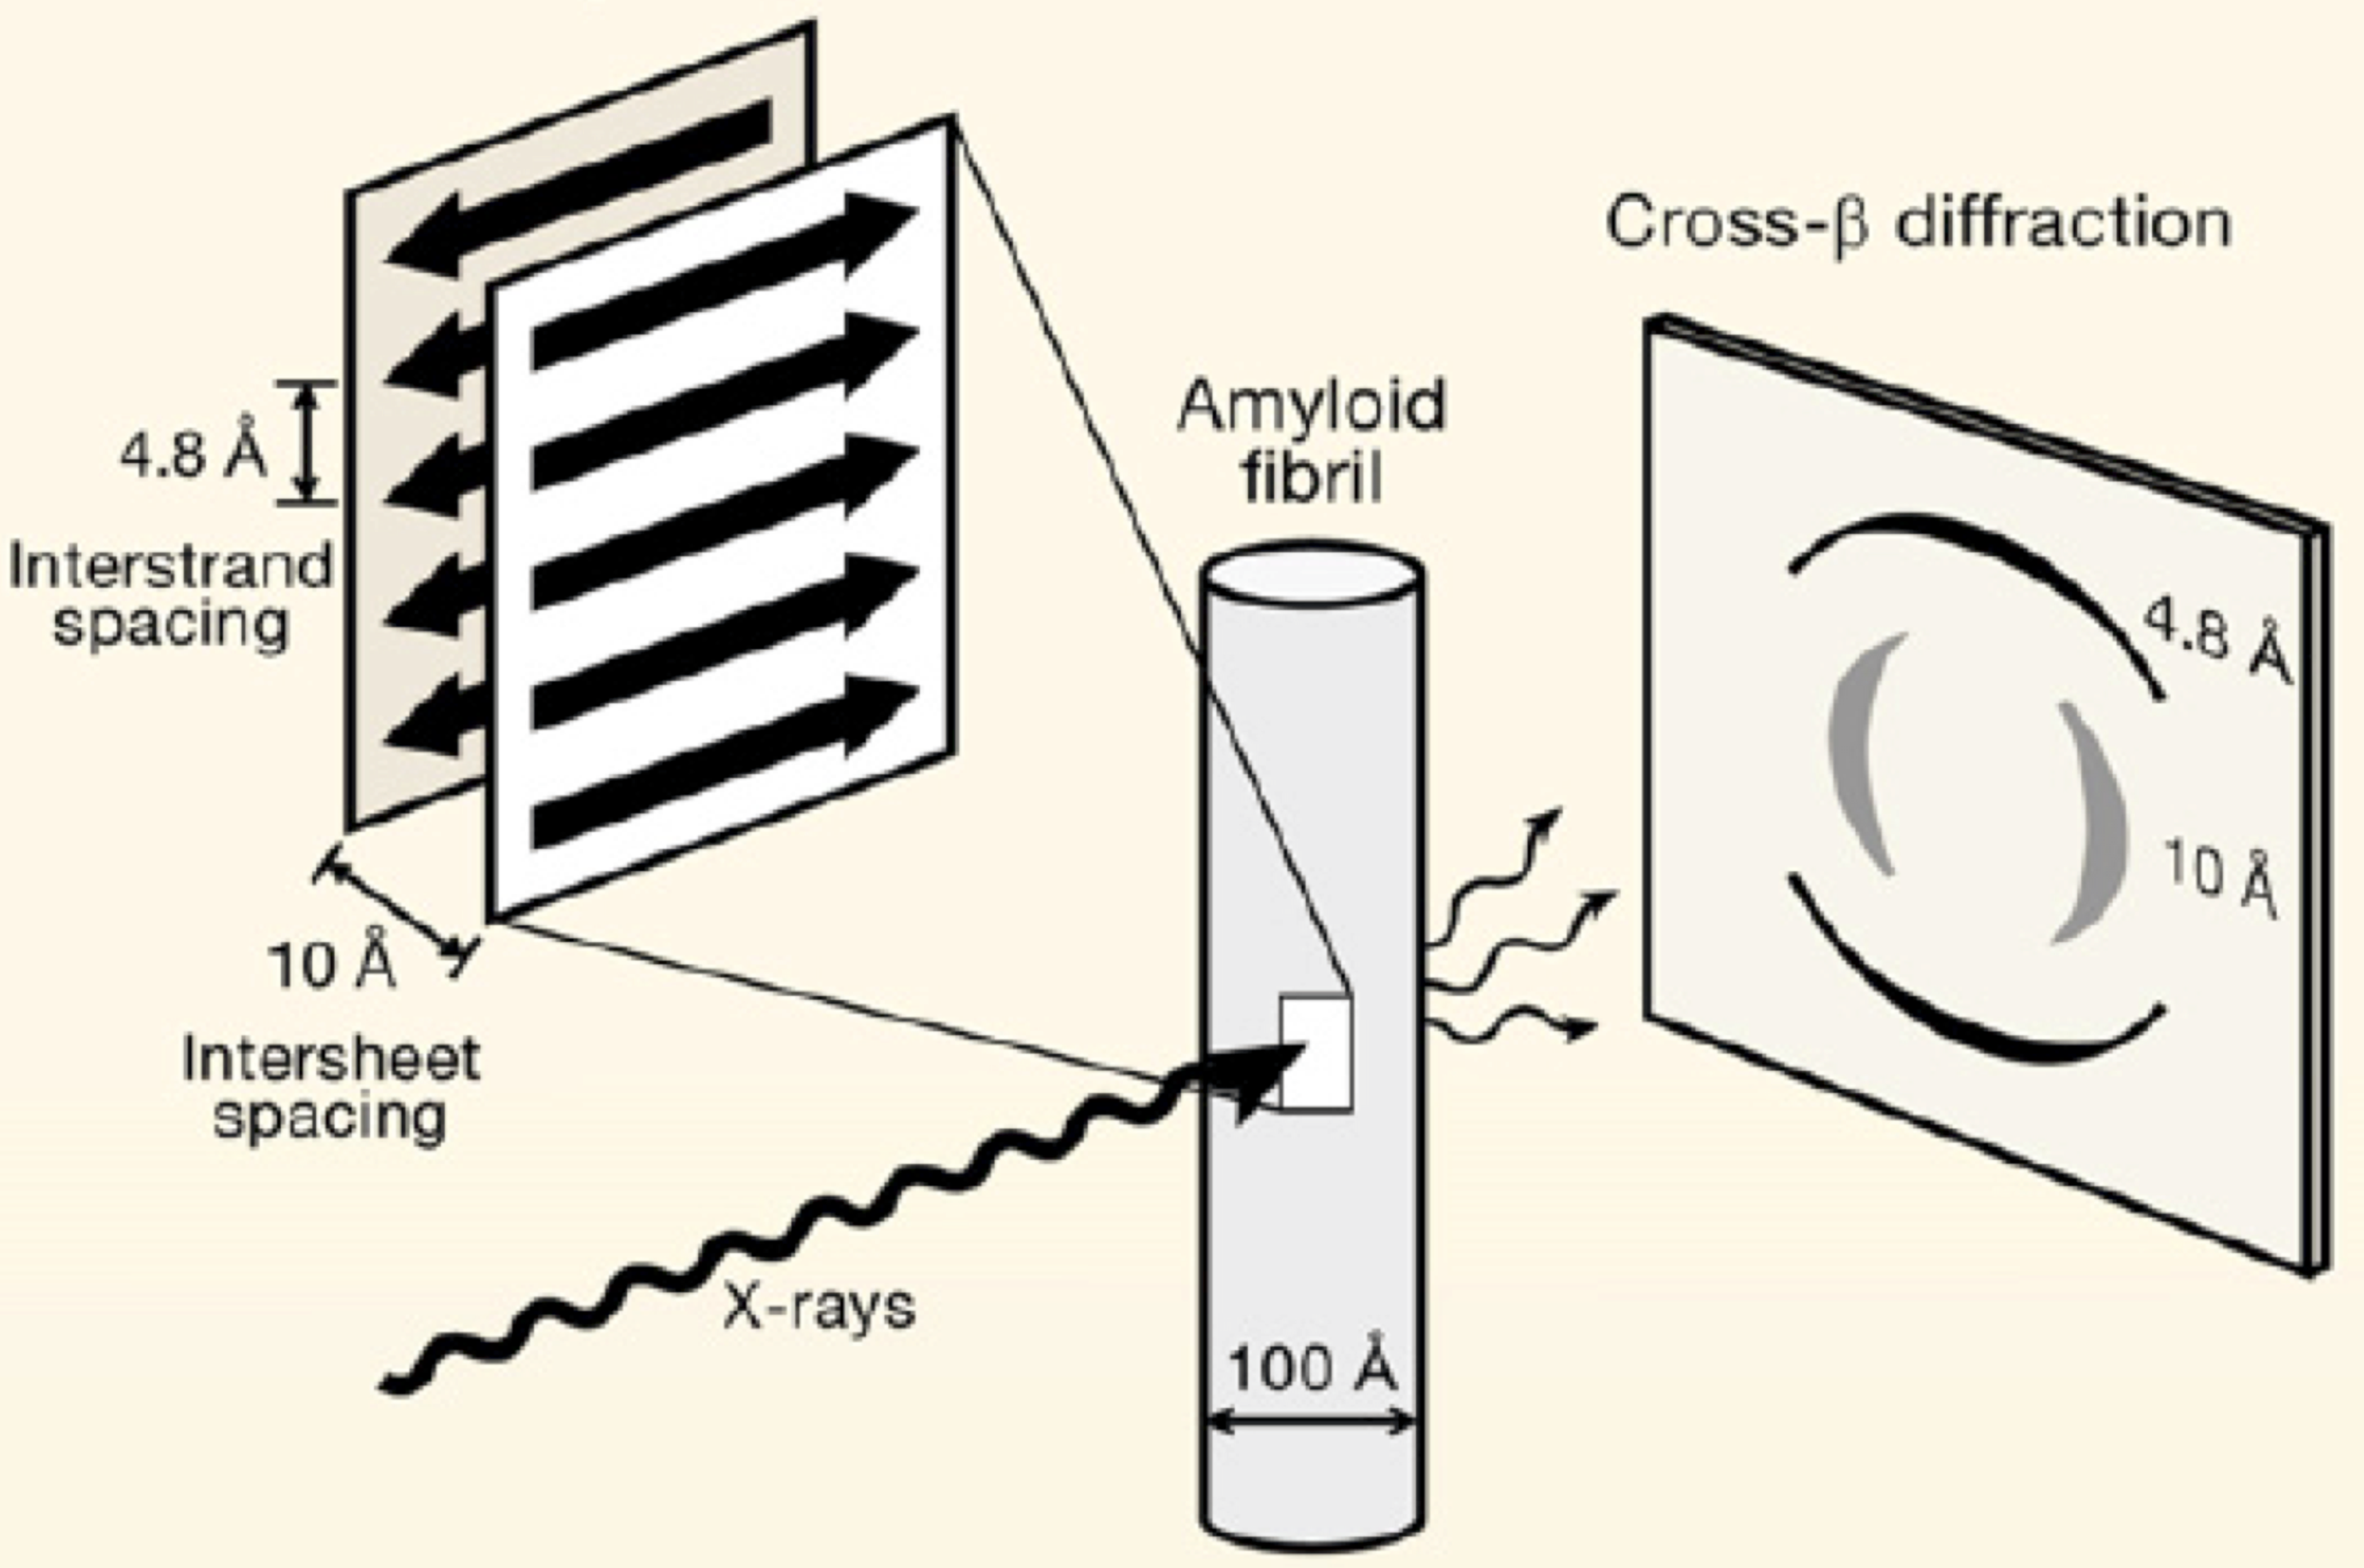
\includegraphics[width=6in]{figures/introduction/fibril_structure_diffraction.pdf}
 \caption[Characteristic cross-$\beta$ spacings from X-ray fibre diffraction studies of amyloid fibrils]{A schematic of the \crossbs\ and the fibril diffraction pattern from X-ray fiber diffraction studies of amyloid fibrils. Adapted from Eisenberg, 2012}
 \label{fig:fibril_diffraction}
\end{figure}

Despite having dramatically different sequences, amyloid fibrils formed from different polypeptides all adopt a similar morphology known as the \crossbs. To date, independent measurements of fibrillar structure from different instruments have all confirmed the cross-$\beta$ as the core structure of amyloid fibrils. Initial structural studies of fibrils using X-ray fiber diffraction showed that their diffraction patterns are characterized by two major orthogonal reflections: meridional and equatorial directions,  corresponding to a 4.8 \angstrom\ interpeptide separation parallel to, and a 10 \angstrom\ intersheet separation perpendicular to the long axis of the fibril, respectively (Figure~\ref{fig:fibril_diffraction}). This diffraction pattern is now considered as indicative of the presence of \crossbs, and hence, of amyloid fibrils. Correspondingly, under the transmission electron microscope (TEM), fibrillar structures are visible as long, unbranched, and ribbon-like structures with diameters between 50 - 100 nms (Figure~\ref{fig:fibril_TEM_SSNMR}). 
% Other measurements? - MPL Mass per unit length?

% Although \crossb\ is widely known, due to the insolubility and inherent non-crystalline nature of amyloid fibrils, the molecular details of the fibril structure remained elusive until recent years. 
% The ubiquitous presence of a \crossbs\ supports that the organization of the peptidic backbone, common to all proteins, in to \bsheets\ is a major determinant of the fibrillar structure. 

\begin{figure}
 \centering
 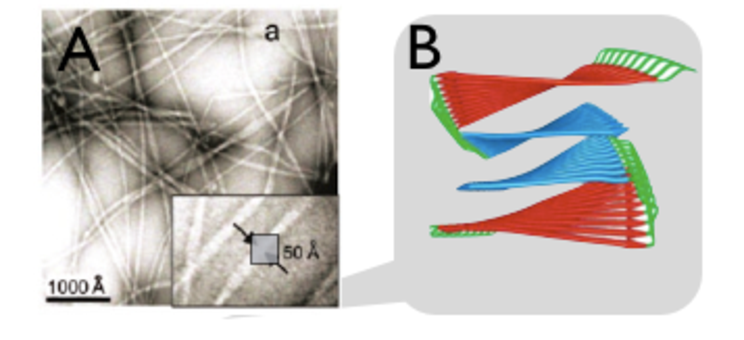
\includegraphics[width=6in]{figures/introduction/fibril_TEM_SSNMR.pdf}
 \caption[Example EM images of non-fibrillar oligomers]{(A) EM image of oligomers of \abeta40\ adapted from Bitan G. et al. 2003 and Walsh D. 1999. (B) SSNMR model proposed by Tycko et al. \textbf{ADD the fibril axes.}}
 \label{fig:fibril_TEM_SSNMR}
\end{figure}

\begin{figure}
 \centering
 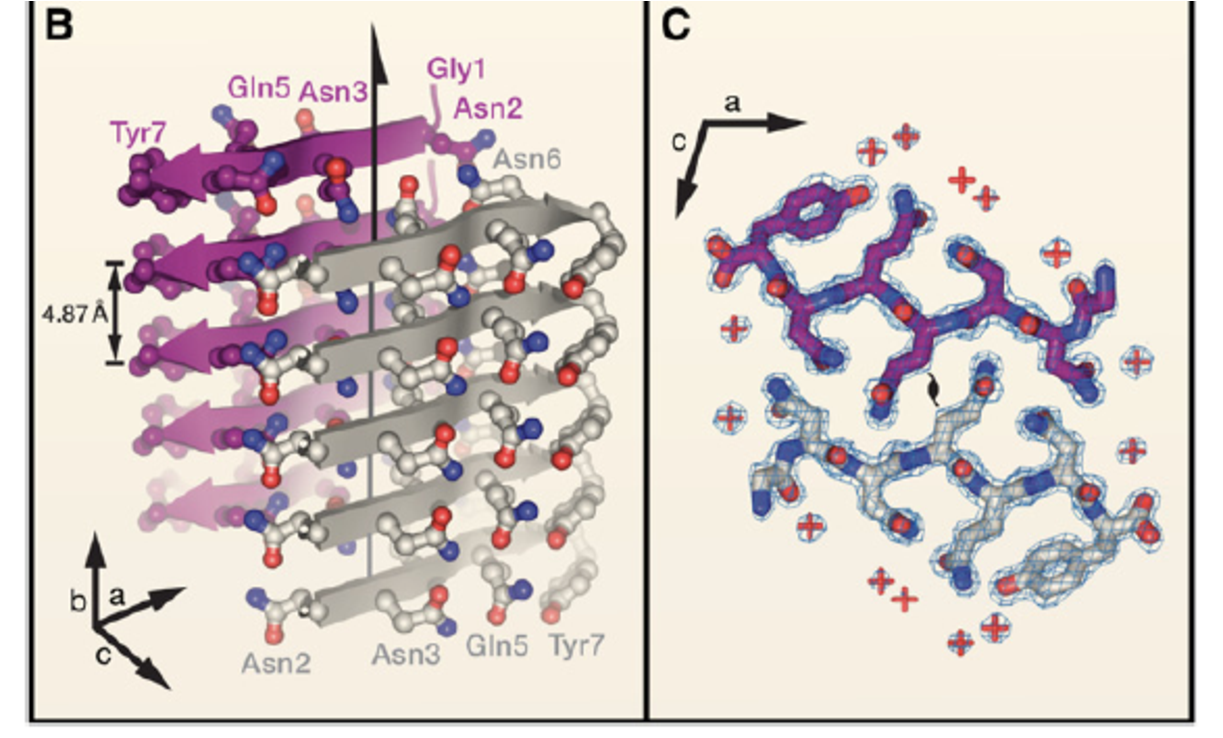
\includegraphics[width=6in]{figures/introduction/fibril_xray_model.pdf}
 \caption[X-ray crystal structure of an amyloid fibril]{A schematic of the X-ray crystal structure of fibrils from from shorter peptide fragments. Adapted from Eisenberg, 2012}
 \label{fig:fibril_xray_model}
\end{figure}

% Describe the molecular structure of \abeta\ amyloid fibrils. Briefly mention the techniques that can be used to obtain structural information of amyloid fibrils. 

% SSNMR
Advances in solid-state NMR (SSNMR) and X-ray crystallography in the last decade have elucidated the molecular details of amyloid fibrils. One of the early SSNMR model of an amyloid fibril was of the \abeta40\ peptide, a protein implicated in Alzheimer's Disease.\cite{Petkova:2006gx}
%The study by Petkova et. al.\cite{Petkova:2006gx} indicated that the \bsheet\ core of \abeta40\ involves residues 10-22 and 30-40, and is linked by a loop formed by residues 23-29. 
The core fibril unit consists of a parallel in-register \bsheet, where each strand is a \bhairpin\ with peptide-peptide backbone hydrogen-bond running parallel to the long axis of the fibril (Figure~\ref{fig:fibril_TEM_SSNMR}). 

Moreover, smaller fragments of A$\beta$ have been shown to form fibrils that are morphologically similar to those of the full length peptide. For example, SSNMR studies of the fibrils of KLVFFAE or A$\beta$(16-22), the central hydrophobic core of A$\beta$, showed that the protofilaments are composed of stacked antiparallel $\beta$-sheets.\cite{Balbach:2000vf} Furthermore, some of these peptide fragments formed amyloid fibrils that were amenable to single crystal X-ray diffraction analysis.  These crystal structures showed that fibrils formed from these shorter peptide fragments are composed of multiple layers of \bsheet\ with a dehydrated (``dry'') stacking interface (Figure~\ref{fig:fibril_xray_model}).\cite{Sawaya:2007p4363}
%Taken together, these recently proposed structures demonstrate that the core region is composed of two to four sheets that interact closely with each other. % I don't think I will talk about the twisting of the sheets too much. Should I mention twisting?

% Fibril polymorphism
Depending on the experimental conditions under which they are formed, fibrils may exhibit polymorphism: the length of the $\beta$-strand involved, side chain orientation and inter-protofilament packing may vary.\cite{Kodali:2007cz} Fibril polymorphism may have important implications in amyloid diseases because, depending on which residues are exposed at the surface, different morphologies may have differing toxicities. For example, in vitro, quiescently formed fibrils of A$\beta$(1-40) have been shown to be more toxic than agitated fibrils.\cite{Petkova:2005p4688} 

% A polymorphic structure introduced by a seed have been shown to be able to propagate in vitro.\cite{Paravastu:2006p4690} A recent study propagated a brain-derived fibril fragment in order to obtain structural information on fibrils that most closely resembles those formed in the AD brain.\cite{Paravastu:2009fi} -- These points aren't going anywhere.

% http://onlinelibrary.wiley.com/doi/10.1111/j.1742-4658.2010.07888.x/abstract?systemMessage=Wiley+Online+Library+will+be+disrupted+on+15+December+from+10%3A00-12%3A00+GMT+%2805%3A00-07%3A00+EST%29+for+essential+maintenance

\subsection{Non-fibrillar oligomers}

Due to their structural disorder and transient nature, obtaining high resolution structural details of amyloid oligomers using traditional structural determination techniques have been impeded.  Unlike fibrils, amyloid oligomers adopt a wide spectrum of structural states. EM and AFM experiments have shown that transient, unstable particles may appear prior to the formation of fibrils.\cite{Chromy:2003p2575,Ahmed:2010p5694,Caughey:2003jq}
% \textbf{ADD: Oligomers formed from amyloidogenic peptides such as $\alpha$-synuclein, etc have also been studied. Do the oligomers formed from different peptides differ?}
Oligomers transient in the fibrillation pathway are known as on-pathway, whereas those that do not progress form fibrils are referred to as off-pathway.\cite{Kayed:2003en} Off-pathway oligomers are typically formed in the presence of detergents, lipids, and certain small molecules.\cite{Yu:2009p2873,Laurents:2005ki} 
% Currently, the precise mechanism involved in the transition from oligomers to extended amyloid fibrils is not known.

Oligomers have been shown to be able to adopt a range of sizes and morphologies. Size exclusion chromatography (SEC) studies of \abeta40\ oligomers (isolated in vitro and from brains of AD patients) showed dimers to large oligomers with hundreds of peptides.\cite{Haass:2007db,Walsh:2007fu} In particular, oligomeric assemblies that are annular, spherical, or curvilinear in shape have been reported in literature.\cite{Haass:2007db,Kim:2009fc,Lashuel:2002eg}

% References for the morphologies from Pat's thesis introd -- (Janson et al. 1999; Conway et al. 2000; Lashuel et al. 2002)
%Conway, K. A., Harper, J. D. and Lansbury, P. T., Jr. (2000). Fibrils formed in vitro from alpha-synuclein and two mutant forms linked to Parkinson's disease are typical amyloid. Biochemistry, Vol. 39, No. 10, pp. 2552-63.
%Conway, K. A., Lee, S. J., Rochet, J. C., Ding, T. T., Williamson, R. E. and Lansbury, P. T., Jr. (2000). Acceleration of oligomerization, not fibrillization, is a shared property of both alpha-synuclein mutations linked to early-onset Parkinson's disease: implications for pathogenesis and therapy. Proceedings of the National Academy of Sciences of the United States of America, Vol. 97, No. 2, pp. 571-6.
%Janson, J., Ashley, R. H., Harrison, D., McIntyre, S. and Butler, P. C. (1999). The mechanism of islet amyloid polypeptide toxicity is membrane disruption by intermediate-sized toxic amyloid particles. Diabetes, Vol. 48, No. 3, pp. 491-8.

% This was directly copied from Fandrich 2012
Oligomers formed from different polypeptide sequences display similar activities in cell metabolic assays,\cite{Bucciantini:2002un} and many share the ability to interact with an oligomer-specific antibody.\cite{Kayed:2003en} % Large spherical oligomers (3-10nm in diameter) formed from disparate sequences have been shown to binding to a single antibody, which suggests that they may share similar structural elements.
Although there is evidence for common properties within some oligomers, unlike fibrils, the secondary structural characteristics of oligomers vary substantially and do not possess a generic structural element. Oligomers have been suggested by many studies to possess high $\beta$-sheet content,\cite{Chimon:2007du,Ahmed:2010p5694,Campioni:2010hz} and may also bind dyes Thioflavin T (ThT) and Congo Red (CR).\cite{Walsh:2007fu,Haass:2007db,Kodali:2007cz}  Moreover, large non-fibrillar oligomers may contain \crossb\ like fragments.\cite{Walsh:2010p4761,Stroud:2012dp,Chimon:2007du} For example, recent structural data from SSNMR studies of Abeta(1-42) suggests that prefibrillar oligomers share common features with the fibrillar forms of A$\beta$.\cite{Chimon:2007du}
% Although oligomers particles may be \bsheet-rich, they are morphologically distinct from fibrils (Figure~\ref{fig:oligomers}).\cite{Walsh:2009p1235}.  % And may contain random-coil-like conformations\cite{Sandberg:2010ix}

%\begin{figure}
% \centering
% 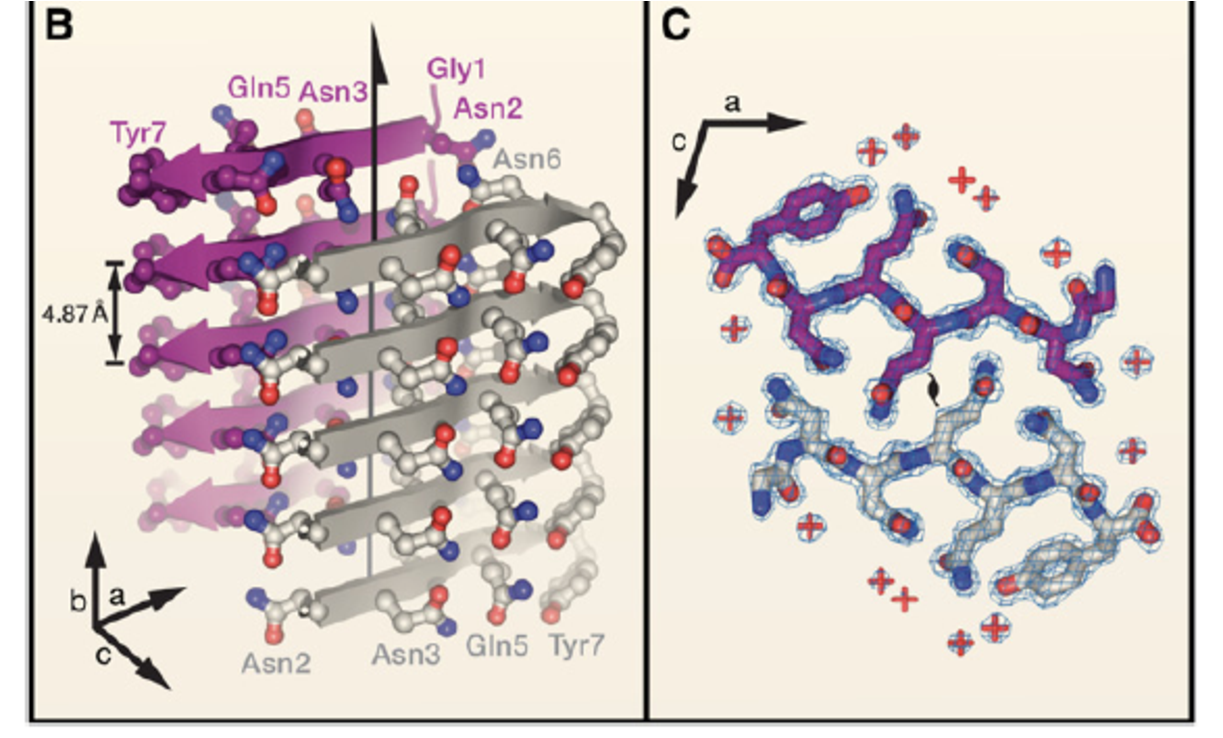
\includegraphics[width=6in]{figures/introduction/fibril_xray_model.pdf}
% \caption[Characteristic cross-$\beta$ spacings from X-ray fibre diffraction studies of amyloid fibrils]{What is this figure suppose to be??}
% \label{fig:fibril_xray_model}
%\end{figure}

%\begin{table}%\footnotesize
% \begin{center}
% \vspace{10pt}
% \caption{Summary of proteins which form amyloids}
% \label{tbl:amyloid_diseases}
%  \begin{tabular}{| c | c | c | c |}
% \hline
% Peptide & Study & fibrils & oligomers \\
% \hline
% \abeta\ & REFs & yes & yes \\
% alpha-synuclein & REFs & yes & yes \\
% \hline
%  \end{tabular}
% \end{center}
%\end{table}

% Amyloid disorders other than AD -- In addition to AD, other neurodegenerative diseases have been shown to involve the presence of amyloid. Parkinson's disease, Huntington's, Prion disorders (Mad cow). These diseases and their pathology are reviewed elsewhere and are beyond the scope of the thesis. In this thesis we focus on AD.

% Outline some of the ideas / hypothesis about the link between amyloid and disease, but don't go into what people speculate or data on toxicity. It is related, but this is out of the scope of your thesis.

% Although not the focus of this thesis, understanding the mechanism of toxicity and elucidating the underlying toxic species will be important in the development of future drug candidates.
%Papers talking about the links of oligomers to disease\cite{Lansbury:2006p928,Lashuel:2006co}
\section{Amyloid involvement in diseases}

Because many diseases were found to have amyloid pathologies in common, it was initially hypothesized that fibrils found in amyloid plaques may be the toxic species in amyloid disorders. However, recent research has implicated soluble oligomers as the likely toxic agent in several neurodegenerative diseases, and type II diabetes.\cite{Haass:2007db,Xue:2009da} % Small non-fibrillar oligomers were found to correlate better with loss of neuronal function (Baglioni 2006) for  Alzheimer's, Parkinson's, Huntington's, Prion diseases.
Currently, the molecular mechanism of toxicity caused by amyloid oligomers is not understood, and is an area under intensive research.  Many studies investigated the link between oligomer toxicity and Alzheimer's Disease, due to the well-known pathological link of Abeta amyloid formation to the neurodegeneration in AD.  Oligomers formed from a variety of peptides, including those that are not implicated in amyloid disorders (e.g. lysozyme, $\beta$2-microglobulin, transthyretin) have all showed toxicity, suggesting that the toxicity of amyloid oligomers may be independent of the peptide sequence.\cite{Fandrich:2012kb,Kayed:2003en} Multiple lines of experimental evidence suggest that this generic mechanism of toxicity is due to the ability of oligomers to interact with the cellular membrane.\cite{Martins:2008bz,Walsh:2007fu} It is hypothesized that oligomeric aggregates, by interacting with and disrupting the integrity of the cellular membrane, may ultimately induce cell death.\cite{Fandrich:2012kb} Moreover, the aggregation of amyloidogenic peptides was found to be enhanced on membrane surfaces,\cite{McLaurin:1997wm,Kayed:2004ul,Yip:2002vx} and that membrane-catalyzed fibril formation may induce cellular toxicity.\cite{Yip:2001tl}
% Oligomeric species are more conformationally flexible and less stable than their fibrillar counterparts.
% Some studies have suggested that Abeta oligomers can increase membrane conductance without the formation of channels.
% Should briefly read up on the book chapter by Pat Walsh and cite him
% An exam question might be: How does inositol eliminate toxicity of oligomers?

\section{Alzheimer's Disease}
Alzheimer's Disease (AD) is a devastating neurodegenerative disease that is most common cause of dementia in persons of age 65 or older. Upon examination, the post-mortem brains of AD patients show significant neuronal dystrophy. Pathologically, AD is characterized by the presence of extracellular deposits of senile plaques and neurofibrillary tangles (NFTs), which appear as lesions on stained neuronal tissue under light microscopy (Figure~\ref{fig:AD_tissue_pathology}).

% Pathological characterization
\begin{figure}
 \centering
 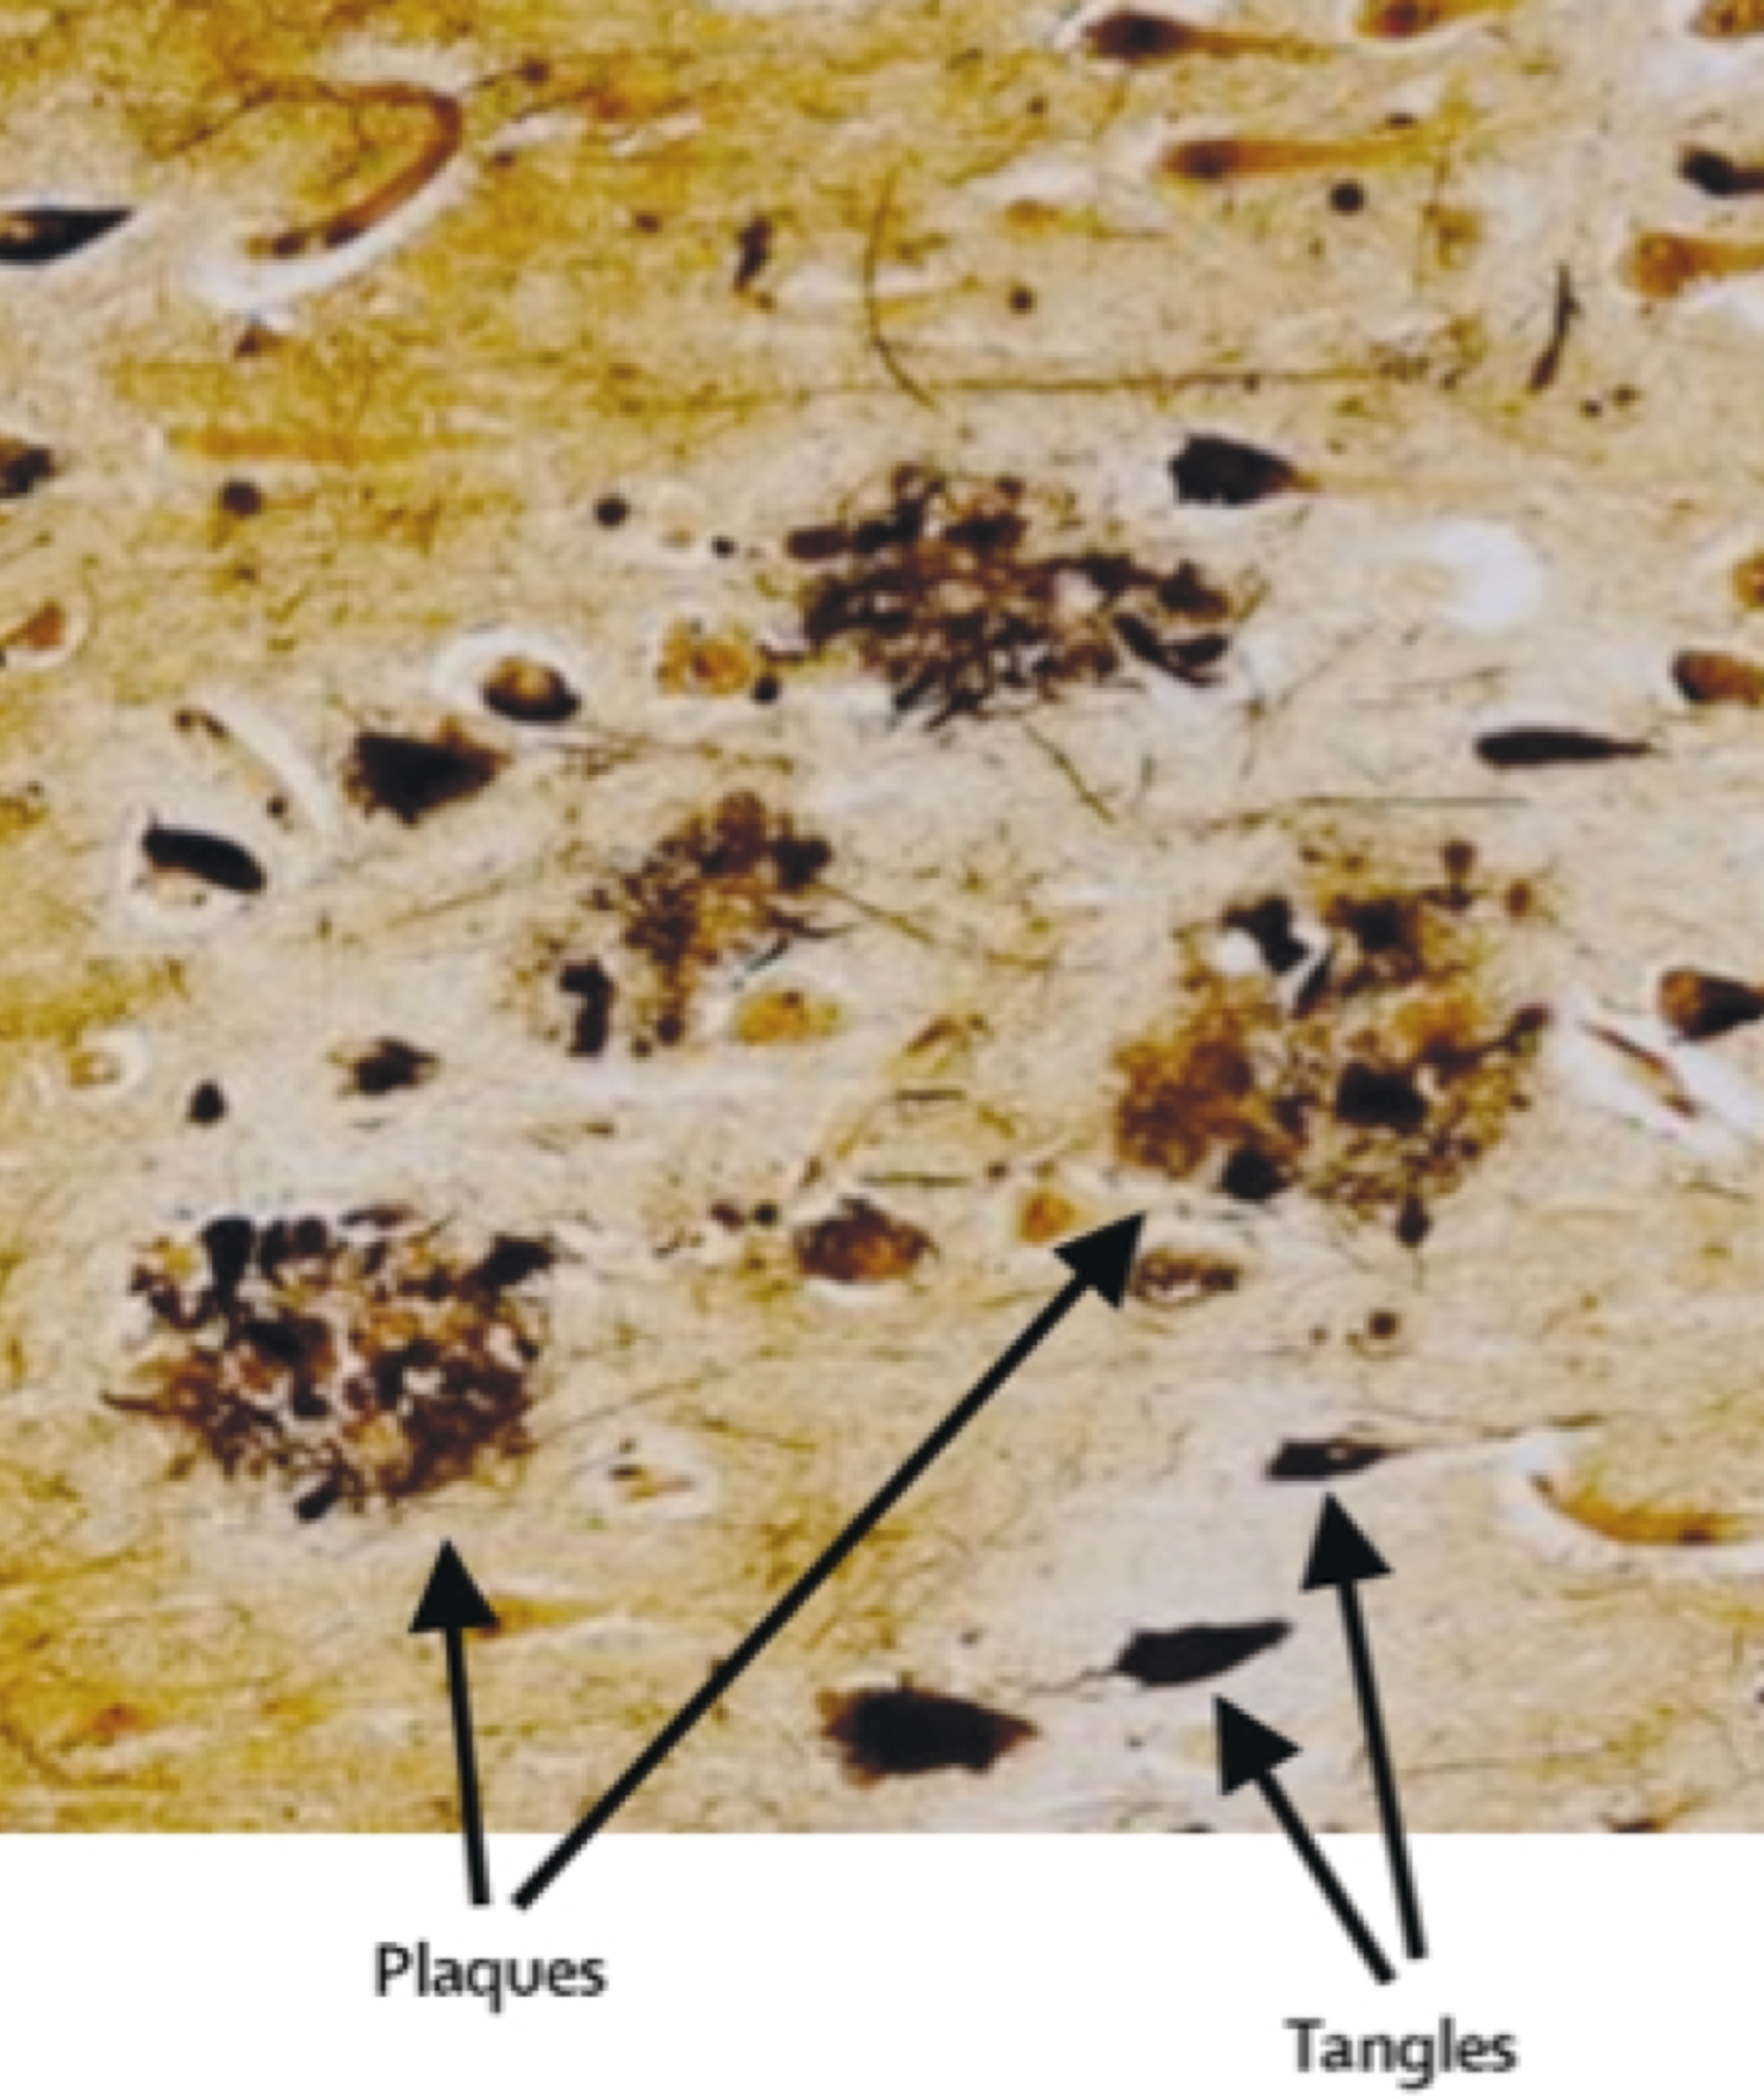
\includegraphics[width=3in]{figures/introduction/AD_tissue_pathology.pdf}
 \caption[AD tissue pathology]{Lesions formed from amyloid plaques and NFT tangles in the cerebral cortex tissue of an AD brain. Adapted from Blennow, 2006}
 \label{fig:AD_tissue_pathology}
\end{figure}

\begin{figure}
\centering
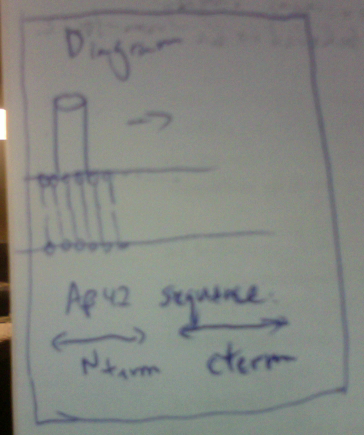
\includegraphics[width=3in]{figures/introduction/AD_abeta_app.png}
\caption[APP processing]{A schematic of the production of A$\beta$ from the amyloid precursor protein.}
\label{fig:AD_abeta_app}
\end{figure}

% Biochemistry of the Abeta peptide.
In 1980s, the amyloid-$\beta$ protein or \abeta\ was identified as the largest component of these plaques. Monomeric \abeta\ is an approximately 4 kDa peptide produced by the intramembrane proteolytic cleavage of the larger amyloid-$\beta$ precursor protein (APP).(Master\'s) \abeta\ is produced constitutively as part of the normal cellular metabolism.\cite{Hardy:2002dh} APP is sequentially processed by the aspartyl proteases $\beta$-secretase and $\gamma$-secretase, where depending on the position of the cleavage by $\gamma$-secretase, a pool of \abeta\ peptides of lengths varying from 38 to 43 residues are produced. (Gandy S) The peptides spanning residues 1-40 (\abetaforty) or 1-42 (\abetafortytwo) are predominantly found in AD-associated plaques. REFS
% Masters CL, Simms G, Weinman NA, Multhaup G, McDonald BL, Beyreuther K. Amyloid plaque core protein in Alzheimer disease and Down syndrome. Proc Natl Acad Sci USA 1985; 82: 4245�49.
% Gandy S. The role of cerebral amyloid beta accumulation in common forms of Alzheimer disease. J Clin Invest 2005; 115: 1121�29.

% Neuritic plaques are composed of mainly \abetafortytwo, whereas \abetaforty\ is more commonly found in cerebral vascular plaques.\textbf{This is out of the blue} 
% Which peptide? Abeta42 or Abeta40
It is currently thought that \abetafortytwo\ is likely to be the more deleterious form of \abeta. (Jarrett) Genetic studies showed that mutations within the presenilin 1 and 2 genes which cause an aggressive early-onset form of AD also leads to an increase in the ratio of \abetafortytwo\ to \abetaforty.\cite{Hardy:1997tu} (Bentahir et al. 2006; Kumar-Singh et al. 2006). Moreover, in vitro, \abetafortytwo\ displays significantly higher propensity for aggregation than \abetaforty, despite differing by only two amino acids.\cite{Barrow:1992vz,Jarrett:1993ti,ElAgnaf:2000vr}

Although it has been more than one hundred years since Dr. Alois Alzheimer first presented the association between the presence of neuronal plaques and the clinical symptoms of presenile dementia characteristic of Alzheimer's disease (AD), the exact relationship between the two is still under much contention.  The ubiquitous presence of amyloid plaque deposits found in the brains of deceased dementia patients led to the formulation of the long-standing amyloid cascade hypothesis, which posits that the amyloidogenesis of \abeta\ plays a key role in the initiation of AD, which ultimately leads to the clinical symptoms of neurodegeneration and dementia.\cite{Hardy:2002dh} Genetic evidence offers strong support for the amyloid hypothesis: in those with trisomy 21 (occurring in Down's syndrome), the chromosome responsible for encoding APP causes the overproduction of A$\beta$ leading to early-onset of dementia with AD-like plaque load. Furthermore, in persons with early-onset familial AD, genetic mutations on the APP lead to the production of A$\beta$ peptides with increased aggregation propensities. % REF -- the biochemistry of AD inside and out.

% Tau protein - Keep discussion brief
In addition to the presence of amyloid plaques, another hallmark lesion found in the brains of patients with AD is intracellular deposition of neurofibrillary tangles (NFTs) composed of aggregated hyperphosphorylated forms of the microtubule-associated protein tau.\cite{Ballatore:2007ir}  % These tau aggregates have a high $\beta$-sheet content that ultra-structurally appears as paired helical filaments (PHFs) (28, 29).\cite{Holtzman:2011gi}
The role of the tau protein and its interactions with amyloid in the pathogenesis of AD are still being established.\cite{Ittner:2010he} Evidence from mouse models currently suggest that the role of NFTs in AD may be downstream to that of \abeta. In particular, \abeta\ production have been shown to drive the formation of tau pathologies: A$\beta$ plaque pathology is not developed in a tau transgenic mouse model, whereas A$\beta$ formation in APP transgenic mice was found to induce hyperphosphorylation of tau.\cite{Gotz:2004dr} 
% Abeta and tau review paper -- \cite{Ittner:2010he}
 % More details on evidence which show that NFTs are not likely the causative species.
% I think this detail about abeta aggregation in vivo is NICE TO KNOW but could be left out of the thesis.
% The concentration of Abeta in the CSF is in the low nanomolar range, but in vitro data shows that the critical concentration for aggregation is in the micromolar range. How does it then aggregate in the brain - mechanism of raising the effective concentration.
% In vitro models have been useful to screen compound libraries for inhibitors of agregation which may have therapeutic efficacy against AD.


\abeta\ aggregates have been found to be present in a variety of morphologies in the brain. Although plaques are often visible in the dementia patients, the plaque load does not correlate with disease progression and severity, a puzzling aspect of AD. Instead, synaptic loss, and severity of cognitive impairment correlated well with the concentration of soluble \abeta\ oligomers in the brain. (Lue et al. 1999; McLean et al. 1999; Wang et al. 1999) Upon the addition of A$\beta$ oligomers (prepared in vitro or extracted from cell cultures), cellullar models of toxicity showed characteristic symptoms of neurotoxicity, leading to eventual apoptosis.\cite{Cappai:2007bc,Lambert:1998ve,Walsh:2002p2566,Shankar:2008bg,Walsh:2007fu} Moreover, injection of certain forms of Abeta oligomers into brains of rats\cite{Lesne:2006gx,Cleary:2005kt} and mice\cite{Martins:2007bz} have been shown to induce neuronal deficits.
% For example, an oligomeric A? species, termed A??56, purified from the brains of mice in an AD mouse model, was found to disrupt memory functions when administered to young rats.
% Lipids have been used to disassemble A? fibrils into smaller structures, which were seen to be highly active in mice.100 
% SUMMARIZE SOME Toxicity EXPERIMENTS HERE. Key studies which lead to the toxicity mechanisms. Pull some from\cite{Fandrich:2012kb}

Although the structures of these soluble oligomers are not determined, studies of the brain-extracts Kuo et al. (1990) of these oligomers suggest that these oligomers are nonfibrillar in conformation (often referred to as ``diffuse'' plaques).\cite{Walsh:2007fu} For example, oligomers extracted from AD brain potently impair synapse structure and function (5). The smallest of these oligomers appears to be dimeric (5). \cite{Roychaudhuri:2009iq} Taken together, current experimental evidence indicates that preventing the formation of these toxic oligomeric forms of A$\beta$ may be a viable method of treatment for AD.

% Other review papers for abeta oligomers \cite{Roychaudhuri:2009iq,Sakono:2010kw}
% SDS- stable low-n oligomers of Ab are the fundamental building blocks of insoluble amyloid deposits and could be the earliest mediators of neuronal dysfunction.\cite{Walsh:2007fu}
% Evidence for the involvement of soluble, non-fibrillar Ab in AD has been gleaned through four distinct experimental approaches that utilize (i) synthetic Ab peptides; (ii) cell culture systems in which APP is over-expressed; (iii) APP transgenic mice; and (iv) human CSF and postmortem brain.
% When Ab is deposited and aggregated in a non�b sheet (nonfibrillar) conformation, it is detected via immunohisto- chemical techniques as �diffuse� plaques (Fig. 1C). REF


% Jarrett JT, Berger EP, Lansbury PT Jr. The carboxy terminus of the beta amyloid protein is critical for the seeding of amyloid formation: implications for the pathogenesis of Alzheimer�s disease. Biochemistry 1993; 32: 4693�97. 
% Walsh DM, Selkoe DJ. Deciphering the molecular basis of memory failure in Alzheimer�s disease. Neuron 2004; 44: 181�93.

% In addition, \abetaforty\ and \abetafortytwo\ also have distinct aggregation pathways in vitro: \abetafortytwo\ is found to form a morphologically more diverse population of intermediate oligomers than \abetaforty.\cite{Bitan:2003ut} 

% What about mice studies? LOOK AT DAVIS THESIS FOR MORE REFERENCES THERE IN SUPPORT OF ABETA42

% Soluble oligomers - structure? toxicity on cells? rats? mouse?
% What kind of an effect do they have? Synaptic toxicity.
% + REFs

% Take a look at how Lemkul covers this section and transitions to it.
% In this section, I will provide an overview of some of the challenges to overcome when developing a small molecule therapeutic for Alzheimer's disease. Furthermore, using this information, I will motivate why inositol is an exciting avenue to explore.
% Briefly mention non-small molecule putative therapies which also acts via amyloid inhibition. The focus of this thesis will be on small-molecule amyloid inhibition.
% Amyloid inhibition as a treatment for Alzheimer's disease and related amyloid disorders. 
% Talk about how important it is to develop drugs for these amyloid disorders 
\section{Amyloid Inhibition by small molecules: A promising method of treatment for AD} 

With the longevity of our population, AD is approaching epidemic proportions with no cure or preventative therapy available.\cite{Blennow:2006wd} In 2010, there are an estimated 36 million people in the world currently suffering from AD, and this number is projected to grow to 115 million people by the year 2050.\cite{alzreport:2012} Furthermore, there are no drugs which may target the underlying disease: approved treatments today such as donepezil (a cholinesterase inhibitor), and memantine (a N-methyl-D-aspartate antagonist) only mitigates cognitive symptoms. REF
% \cite{Mangialasche, F. M., Solomon, A., Winblad, B., Mecocci, P., and Kivipelto, M. (2010) Alzheimer’s disease: clinical trials and drug devleopment’. Lancet Neurol. 9, 702�716.} \cite{(4) The 2012 PhRMA Report on Medicines in Development: Alzheimer’s disease. See www.phrma.org.} 

% PhRMA reports in their 2012 Medicines in Development Report for AD4 that there are currently 93 medicines in various stages of development, both small molecule and biologic. In general, all 93 compounds fall into one of the following therapeutic strategies: (1) agents targeting neurotransmission, (2) agents targeting Aβ production, (3) agents targeting Aβ aggregation, (4) agents targeting Aβ clearance, (5) agents increasing brain resistance to Aβ, (6) agents targeting tau protein, and (7) agents targeting neurotrophins and agents modulating synaptic plasticity and nerve growth.1−4 \cite{From the ACS neurochem's editorial letter}

% (1) Data from the Alzheimer’s association. See www.alz.org.
% (2) Data from Alzheimer’s foundation. See www.alzfdn.org.
% (3) Mangialasche, F. M., Solomon, A., Winblad, B., Mecocci, P., and Kivipelto, M. (2010) Alzheimer’s disease: clinical trials and drug devleopment’. Lancet Neurol. 9, 702−716. Special Issue: Alzheimer's Disease Published: November 21, 2012
% (4) The 2012 PhRMA Report on Medicines in Development: Alzheimer’s disease. See www.phrma.org. -- I should have a look at this report
% (5) Sadeghi-Nejad, N. (2012) The Lessons of failure: what we can learn from bapineuzumab’s blowup. Forbes (Pharma & Healthcare), August 7, 2012.
% (6) For information of the clinical trials with MK-8931, see www. merck.com.

\textbf{Need to funnel down to sm inhibition.} Hence, it is imperative that efforts be made towards the development of therapeutics for AD. The vast number of structural and biochemical studies on amyloid structure have been crucial for the development of potential therapeutics for treating the underlying disease. A promising method of treatment of AD is by preventing amyloid aggregation, and decreasing amyloid production have gained traction in recent years. A detail review of different method of treatments, which targets the underlying disease is provided elsewhere.\cite{Salomone:2012fh}

%Small molecules which prevent amyloid formation may be an effective method of treatment for amyloid disorders because of the potential to treat the underlying disease. 

\textbf{Explain the desirable traits of a drug for AD, and the pharmacological challenges which finding a small-molecule inhibitor of AD presents.} A key pharmacological challenge of developing a drug for AD and other neurodegenerative diseases involves developing a small molecules with the ability to penetrate the blood-brain barrier (BBB) to achieve sufficient concentrations in the brain for their therapeutic effects (ie. to inhibit amyloid formation). % Expand on this paragraph?
% Concentration at which the small molecule acts. BBB penetration and bioavailability.
In recent years, in vitro screening has led to the discovery of a large number of small-molecules which were found to affect the amyloid aggregation pathway. REF Some inhibited amyloid fibrils, whereas others arrested or reduced non-fibrillar oligomer formation. Many of these small molecules are thought to act by directly binding to amyloidogenic peptides and aggregates. REF The main classes of molecules that have demonstrated promise as amyloid fibrillation inhibitors are reviewed in the sections below.
% Note that here I can take a cue from Justin Lemkul`'s recent review paper.

\begin{figure}
\centering
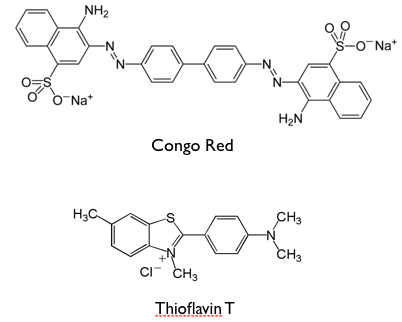
\includegraphics[width=3in]{figures/introduction/dyes.png}
\caption[Amyloid-binding dyes]{Chemical structure of amyloid-binding dyes congo red and thioflavin T}
\label{fig:amyloid_dyes}
\end{figure}

% Questions to answer for the sections below on the various small molecule inhibitors.
% Is it specific to Abeta amyloid inhibition? Or fibril structure or what? 
% Any measured concentration of acitivity, IC/EC50, Kd of binding?
% Biophysical data of binding and whether they've been adapted into a drug or were there attempts made to adapt into a drug.
% Molecular mechanism of binding of dye molecules. Thought to bind flat on on the surface grooves of amyloid fibrils where they interact with hydrophobic groups exposed at the surface. 
 % Doesn't explain why the dye molecules are also able to suppress fibril formation.
 % What they are used for ... why one is used over the other. Contrast binding modes, and binding mechanisms, and binding constants. 
 % Make this section tight. Lots of repeat information. Lots of confusing data. Lots of biophysical characterization but still no exact mechanism.
 % Question: Can the birefringence be explained by these binding modes? -- this is out of the scope of my thesis. Don't put this in my thesis but I should be able to coherently explain this during my defense.

% Congo Red (CR) -- DISCUSS ITS PUTATIVE BINDING MODES with amyloid fibrils. What are some binding measurements IC or EC50 values? micro molar? milimolar?

\subsection{Dye molecules}

Among the first molecules known to bind amyloid fibrils were dyes molecules used to identify their presence (Figure~\ref{fig:amyloid_dyes}). Early histological detection of amyloid binding was done using congo red (CR), where upon binding with CR, fibrils exhibit red-green birefringence when viewed with polarized light.\cite{Frid:2007bo} The binding affinity of CR to various fibrils are estimated to be in the range of 0.1 - 1.5 micromolar. \textbf{detailed studies}.\textbf{Putative binding modes of CR molecules with the amyloid fibril are most likely to be bound along the long axis of the fibril. Binding studies where chemical modifications to CR suggest that both ionic and hydrophobic interactions may be important for its binding as disruption of either can affect its binding affinity.  Although CR is typically used to detect the presence of fibrillar aggregates, CR may also interact with non-fibrillar conformations such as monomers of alpha-synuclein, and alpha-helical form of poly-L-lysine}.\cite{Maltsev:2012kw} 

Early studies \textbf{what kind of studies?} of amyloid using CR led to the finding that CR not only binds to fibrils, but also affect the amyloid aggregation pathway by interacting with one or more amyloidogenic species.\cite{Caspi:1998vt}  CR may inhibit and promote amyloid formation in a dosage-dependent manner: Fibril formation of amyloidogenic proteins Abeta,\cite{Esler:1997bq} prion,\cite{Rudyk:2000ta} and immunoglobulin light chain variable domain (SMA)\cite{Kim:2003hv} were found to be promoted by the presence of CR at low molar ratios, and inhibited at high molar ratios. 
% \textbf{Not sure if this idea belongs here} Furthermore, it can also self-aggregate in solution to form complexes, which may play a role in its binding mechanism to amyloid peptides and aggregates.\cite{Maltsev:2012kw,Lendel:2009cg}
% Study on CR which shows that it can interact with ThT to interfere with amyloid detection \cite{Buell:2010p9457}

Although CR exhibits anti-amyloidogenic and anti-prion properties, it has low penetrability through the BBB and is carcinogenic, making it a poor therapeutic candidate. Therefore, efforts were applied to find CR-based analogues, which maintain their anti-fibrillar aggregation activities, but with improved toxicity profile and BBB bioavailability. Chrysamine G (CG) is one such analogue of CR with higher lipophilicity than CG, which allows it to cross the BBB, lowered toxicity, and capable of inhibiting aggregation and amyloidogenic toxicity in vitro and in vivo.\cite{Klunk:1994um,Klunk:1998vm,Reinke:2007p155,Ishii:2002uf}
% lipophilic - ``fat-loving''
% Citations
% A Chemical Analog of Curcumin as an Improved Inhibitor of Amyloid Abeta Oligomerization

% Thioflavin T (ThT)
\textbf{Note to self - Not sure if this idea belongs here.  Basically how molecules may bind to amyloids. Consider moving this to the section where I talk about MD simulations ... and combine it with biophysical studies which attempts to elucidate the molecular mechanism of binding ... In anycase, I don't feel like there is any computational studies that offer ``decent'' insight into binding. Also I think talking about binding mechanisms fits better there because I've also introduced ideas of binding equilibria etc.}
The use of congo red to detect the presence of amyloid formation is often a laborious process, and only gives a qualitative measurement of the amount of amyloid present. Thioflavin-T (ThT) is a benzathiole fluorescent dye also used to detect the presence of amyloid fibrils in post-mortem brain tissue samples, and monitor fibril formation in vitro. ThT exhibits a dramatic shift in the excitation spectrum maximum and an emission enhancement upon binding to fibrils, making it a sensitive and efficient report for the presence of amyloid fibrils. ThT is soluble in water and have \KD\ in the low \micromolar\ range: 0.033 to 23 micro molar.\cite{Groenning:2009p2723}

\textbf{Is ThT binding similar to CR's ?} Due to the ubiquitous use of ThT as a amyloid fibril probe, fibril binding by ThT is well-characterized. Studies have suggested that ThT binds at the surface of the fibril, parallel to its long-axis, and may depend on the physiochemical properties of the amyloid fibril. \cite{Wu:2009p1954,Biancalana:2010p5053,Wu:2011fd,Mao:2011ic} More than one binding site with similar affinities for ThT may be present on fibrils. Moreover, ThT binding is not limited to fibrils, and was found to bind in hydrophobic pockets of human serum albumin, a globular protein, with comparable affinity to many drug-like molecules.\cite{Groenning:2007p3436,Groenning:2007eo}
% Question - Does ThT affect aggregation as well? The review paper by groenning mentions that it doesn't ... but check again. Should mention here. 
% Question - How does ThT bind? And what causes the fluorescence upon binding?
% ThT fluorescence is only observed from those molecules that have bound to the fibrils, where they exhibit a shift in the excitation spectrum maximum, from 385 nm to 450 nm, and the emission maximum, from 445 nm to 482 nm.  
% Which binding modes can explain ThT's excitation spectrum upon binding? Firstly, steric and electronic stabilization (via charge transfer) of the ground-state charge distribution (7,8); and 2), restriction in the rotation of the aromatic rings of the dye (see Fig. 1 A) in its electronically excited state (9,10).\cite{Wu:2011fd}} -- I think this is out of the scope of my thesis. I could get asked on this. Learn it but don't write it in.

% Other dye-based inhibitors:
% Methylene Blue is a histological dye molecule (which dye is it based on?) shown to promote the fibrillation of Abeta.
% According to Joanne, it is coming back in clinical trials -- I don't think I need to include this here.
% http://www.ncbi.nlm.nih.gov/pubmed/17595112

% Imaging agents -- I think I should also leave this to good to know. I'm not writing a general review here of the uses of different compounds. I'm talking about what we know about the binding mechanism of various compounds for the inhibition of amyloid formation as a therapy for amyloid disorders.
% In addition to the modification of dyes for the development of therapies, dye molecules have also been used as scaffolds to develop new imaging agents.  One such compound is Pittsburgh compound B (PiB), a derivative of ThT, where chemical modifications to ThT led to a much higher binding affinity (in the nanomolar) for amyloid fibrils, and improved BBB penetration.\cite{Raji:2008cv}

% Kill this for now -- Crystallography study of orange-G, a dye-based ...., with amyloidogenic fibril fragments of Tau and Abeta, showed that Orange-G intercalated between sheets by making both nonpolar and electrostatic interactions.\cite{Landau:2011gu}

%\begin{table}%\footnotesize
% \begin{center}
% \vspace{10pt}
% \caption{Summary of small molecules known to affect amyloid formation}
% \label{tbl:inhibitors}
%  \begin{tabular}{| c | c | c |}
% \hline
% Molecule & Study & Mechanism of action \\
% \hline
% ThT & REFs & Binding to fibrils \\
% EGCG & REFs & Binding to toxic oligomers \\
%	 \hline
%  \end{tabular}
% \end{center}
%\end{table}

% Where are they found? Plants, animals, in food. What are they used for in nature?
% Chemical features of polyphenols? Properties? Soluble?
% What is known about their molecular mechanism?
%\textbf{What other diseases can they treat?}
% for AD
% \textbf{summarize some in vitro studies}
% \textbf{summarize some mouse studies}
%\textbf{Their pharmacological properties ... toxicity in the context of treating brain diseases ... }
%\textbf{Has there been any trials using them? Good to indicate here.}
% Curcumin is a flavonoid, resveratrol is not.
\subsection{Polyphenols}
\begin{figure}
\centering
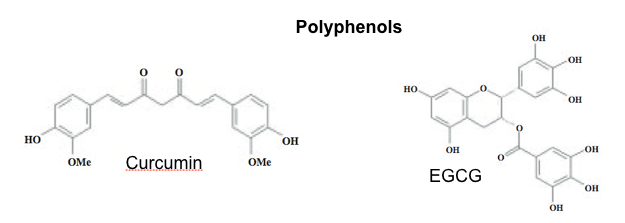
\includegraphics[width=6in]{figures/introduction/polyphenols.png}
\caption[Polyphenol molecules]{Chemical structures of flavonoids curcumin and EGCG. \textbf{\resve\ should also be added here}}
\label{fig:polyphenols}
\end{figure}

Polyphenols is a class of molecules found naturally in plants composed of one or more aromatic phenolic rings, with multiple hydroxyls around these rings.  The consumption of certain antioxidant polyphenols have been reported by many studies to be beneficial for health, such as prevention of cancer, and heart disease.  In recent years, in vitro studies suggest that phenolic compounds may inhibit amyloid formation.\cite{Porat:2006fn}
Here we provided an overview of the phenolic compounds  -epigallocatechin-3-gallate (EGCG), curcumin, and resveratrol, which have been well-studied in recent years for their in vitro activity in preventing amyloid formation.

EGCG is the major polyphenolic component of green tea, and is well-known for its cancer-preventative effects, which are supported by multiple cell culture, animal, and clinical studies.\cite{Singh:2011ec}  In vitro, EGCG molecules promote self-assembly of amyloidogenic peptides \abeta\cite{Ehrnhoefer:2008fd} and \alphas\cite{Bieschke:2010ju} into ``off-pathway'' oligomers and inhibit the formation of mature fibrils by directly binding to monomeric forms of these peptides. Furthermore, in vitro cell culture experiments indicate that micromolar concentrations of EGCG are protective against A$\beta$-induced cell death.\cite{Levites:2003wm,Bastianetto:2006du} Another flavonoid, \cur, the main constituent of the spice turmeric. In vitro, \cur\ inhibited Abeta aggregation with reported IC$_{50}$ values between 0.1-1 \micromolar.\cite{Singh:2012df,Ono:2004td,Hamaguchi:2009p2874,Kim:2005wk}  
% Studies with AD mice models have suggested that \cur\  can penetrate the BBB in AD.REF
% Although this is the case, \cur\ is likely to have poor bioavailability when administered orally:  in rats that were fed \cur\, negligible amounts of the compound were detected in their blood, and high doses were required to attain detectable doses in tissue levels. 

Resveratrol, a polyphenolic molecule found in grapes, red wine and berries, is well-known for its link to the cardioprotective benefits of drinking red wine. Moreover, in vitro and in vivo studies have suggested \resve\ to aid in the treatment of cancer, for which several clinical trials in various are underway.\cite{Baur:2006bx}  In recent years, \resve\ has gained additional attention due to its potential therapeutic effect for treating AD: Resveratrol is found to inhibit the fibril formation of amyloid-$\beta$ and the islet amyloid polypeptide (involved in type II diabetes) in vitro, and thereby attenuating amyloid-induced cellular toxicity.\cite{Ono:2008bl,Feng:2009p2240} % Resveratrol is current under phase II of clinical trials to determine if resveratrol therapy is beneficial in improving the cognitive function in people with AD.
% Experimental studies of several flavonoids, depicted in Figure~\ref{fig:polyphenols},  are able to modulate amyloid aggregation. Because of their favorable in vivo toxicity and high IC50 of inhibition, they have emerged as promising therapeutic candidates for Alzheimer's Disease and related neurodegenerative diseases.

Because of their anti-amyloidogenic activity, low toxicity, and ability to permeate across the BBB, polyphenols have therapeutic potential for the treatment of AD and related neurodegenerative diseases.  Although many in vitro studies suggest that they inhibit amyloid aggregation, their mechanism of action is currently not yet understood. A key disadvantage of polyphenols is their high metabolic activity in the gastrointestinal system, which leads them to be poorly absorbed when administered orally.\cite{Baur:2006bx,Smith:2011iq,Hamaguchi:2010wu} Phase I and Phase II clinical trials of  \cur\, \resve\ and EGCG for their efficacy in the treatment of AD are currently underway. 
%Curcumin clinical trials --- Although no adverse events were reported, and the Because these trials only involved a small number of people (between 11 - 34),  the effects of \cur\  on cognitive function are inconclusive.\cite{Hamaguchi:2010wu}

% Do they have all similar mechanism of action in vitro? 
% \textbf{summarize some in vitro studies}
% \textbf{summarize some mouse studies}


%19. Porat Y, Abramowitz A, Gazit E (2006) Inhibition of amyloid fibril formation by polyphenols: Structural similarity and aromatic interactions as a common inhibition mechanism. Chem Biol Drug Des 67(1):27�37.
%20. Ehrnhoefer DE, et al. (2008) EGCG redirects amyloidogenic polypeptides into un- structured, off-pathway oligomers. Nat Struct Mol Biol 15(6):558�566.
%21. Bieschke J, et al. (2010) EGCG remodels mature ?-synuclein and amyloid-? fibrils and reduces cellular toxicity. Proc Natl Acad Sci USA 107(17):7710�7715.
%22. Ladiwala ARA, Dordick JS, Tessier PM (2011) Aromatic small molecules remodel toxic soluble oligomers of amyloid ? through three independent pathways. J Biol Chem 286(5):3209�3218.
%23. Lemkul JA, Bevan DR (2012) Morin inhibits the early stages of amyloid ?-peptide aggregation by altering tertiary and quaternary interactions to produce �off-pathway� structures. Biochemistry 51(30):5990�6009.
%24. Sinha S, et al. (2012) Comparison of three amyloid assembly inhibitors: The sugar scyllo-inositol, the polyphenol epigallocatechin gallate, and the molecular tweezer CLR01. ACS Chem Neurosci 3(6):451�458.
%25. Lopez del Amo JM, et al. (2012) Structural properties of EGCG-induced, nontoxic Alzheimer�s disease A? oligomers. J Mol Biol 421(4-5):517�524.
%26. DeToma AS, Choi J-S, Braymer JJ, Lim MH (2011) Myricetin: A naturally occurring regulator of metal-induced amyloid-? aggregation and neurotoxicity. ChemBioChem 12(8):1198�1201.

%\subsection{Non-steroidal Anti-inflammatory compounds (NSAIDs)}
%% Naproxen and ibuprofen
%% From \cite{Takeda:2010gx,Raman:2009jn}
%CUT THIS SECTION DOWN
%
%% I don't think I need to include a whole paragraph summarizing ibuprofen. It's the same story as inositol.
%One of the potential candidates is a nonsteroidal anti-inflammatory drug (NSAID) naproxen and ibuprofen (\ref{fig:nsaids}).\cite{XXX} Epidemi- ological studies have shown that chronic prophylactic intake of naproxen moderately reduces the risk of AD.12,13 Furthermore, reexamination of the results of large-scale clinical trials suggests that under certain conditions naproxen can reduce the AD risk by 67\%.11
%
%Biomedical studies suggest that treatment with ibuprofen reduces the amount of Ab deposits and alleviates memory deficits in mice models (17,18). Ibuprofen intake also correlates with a decrease in the amount of Ab oligomers in mice brain tissues (18). A prophylactic long-term use of ibuprofen appears to reduce the risk of AD (19), but the effectiveness of this drug against preexisting AD cases is unclear (20). 
%
%Several recent experimental studies have investigated the molecular aspects of interactions between Ab and ibuprofen. Binding of ibuprofen to Ab fibrils has been demonstrated when the ligand/peptide stoichiometric ratio approximates or exceeds 1 (21,22). 
%
%Experimental in vitro studies have shown that ibuprofen reduces accumulation of Ab fibrils by apparently interfering with fibril elongation (23). Furthermore, ibuprofen demon- strates an ability to at least partially dissociate preformed Ab fibrils (21,23).
%
%\begin{figure}
%\centering
%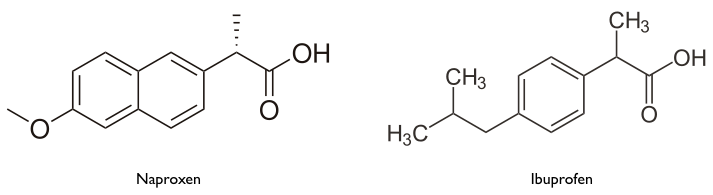
\includegraphics[width=4in]{figures/introduction/nsaids.png}
%\caption[NSAIDs]{NSAIDs}
%\label{fig:nsaids}
%\end{figure}

\subsection{Inositol}
% Here we will review the physiological role of inositol in nature, and introduce inositol as a potential therapeutic for amyloid disorders. Here, use the physiological role of myo-inositol as a lead to transition into its role in amyloid inhibition.
\begin{figure}
	\centering
	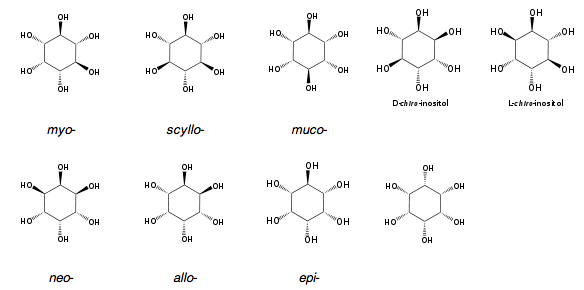
\includegraphics[width=6in]{figures/introduction/inositol.png}
	\caption[Inositol stereoisomers]{The nine stereoisomers of inositol.}
	\label{fig:inositols}
\end{figure}

Inositol with the molecular formula of \ce{C_6H_{12}O_6}, is a class of simple polyols with nine naturally occurring stereoisomers (Figure~\ref{fig:inositols}). Out of these nine isomers, seven are optically inactive, and the remaining two (L- and D-chiro-inositol) are chiral enantiomers (Figure~\ref{fig:inositols}). myo-Inositol, the most abundant isomer, is ubiquitous in all eukaryotes and is a physiologically important osmolyte. Furthermore, myo- is a precursor for inositol lipid synthesis: It is a constituent of phosphatidylinositol, an important phospholipid in membranes and second messenger systems. Once phosphorylated, myo-inositol phosphatides act as second messengers in intracellular signal transduction pathways.\cite{Fisher:2002tk} 
% Add some specific pathways which involves inositol are XXX ... YYY.\cite{Michell:2008dh}

Inositol is found in high concentrations in tissues of the human central nervous system (CNS): myo- And scyllo-inositol have approximate concentrations of 5 and 0.1-0.5 mM in the CNS, respectively.\cite{Fisher:2002tk} Accordingly, inositols also function as osmolytes in the CNS, where alterations in their concentrations are known to be associated with neuropathological conditions.\cite{Michaelis:1993gf, Fisher:2002tk}

% Role of inositol in amyloid inhibition. Here, include the background on how inositol was discovered as an \abeta\ amyloid fibril inhibitor. Should try to make it into a little story of how inositol was discovered. 
In recent years, scyllo-inositol have been identified as a promising therapeutic candidate for the treatment of Alzheimer's Disease. Inositol was initially discovered because of studies of Abeta42 with lipid bilayers composed of acidic phospholipids was shown to induce beta structure in Abeta42.\cite{McLaurin:1996p584} Upon closer examination, myo-inositol the headgroup of phosphatidylinositol was found to be responsible for the induction of $\beta$-sheet structure in monomeric \abeta42.\cite{McLaurin:1998p3976, McLaurin:1998p3149}. Moreover,  fibrils were not formed. This discovery led to the in vitro studies which showed that inositol exhibits stereochemistry-specific effects on \abeta\ fibril inhibition and cytotoxicity. scyllo-, myo-, and epi-, but not chiro-inositol inhibit \abeta42 fibril assembly, stabilize an oligomeric complex of \abeta42, and attenuate \abeta-oligomer-induced neurotoxicity in vitro.\cite{McLaurin:2000bq} In vivo studies with a transgenic mouse model of AD demonstrated that the decrease in their AD-like symptoms after inositol treatment was correlated with a decrease in the levels of soluble \abeta\ oligomers, suggesting that the beneficial effects of scyllo-inositol may be attributed to the inhibition and/or disaggregation of high-order \abeta\ oligomers.\cite{McLaurin:2006eb}

% I think this is an important paragraph, except I'm not entirely clear on An important therapeutic advantage of scyllo-inositol is its ability to readily crosses the blood brain barrier (BBB) (both actively and passively transported). Because it is not enzymatically broken down in the gut, it may be adapted into an orally-administered drug. Although scyllo-inositol is found naturally in certain plant organisms and ..., quantities needed for it to be an effective therapeutic is synthesized inside the body ... or can be obtained via nutrition?

Presently, scyllo-inositol has completed both phase I and II of human clinical trials for the treatment of AD.\cite{Ma:2012jk,Salloway:2011im} Phase I of human clinical trials with a total of 110 healthy participants has been completed. Based on indicators such as brain plasma and CSF concentration levels, scyllo-inositol was found to be non-toxic to healthy individuals at concentrations effective for amyloid inhibition. From 2007 to 2011,  Phase II studies of scyllo-inositol were conducted with three dosage groups, where subjects in each group were administered 250 mg, 1000 mg or 2000 mg of \emph{scyllo}-inositol (ELN005) orally twice a day, where each group was comprised of 84 to 91 subjects. However, because of greater incidences of serious adverse events, in the trials at the two higher dosage, only the lower dose was continued. Due to the decrease in the statistical power of the study from the removal of the two highest doses, the efficacy of scyllo-inositol was not conclusive.\cite{Ma:2012jk,Salloway:2011im} Taken together, these results suggest that scyllo-inositol may be a promising therapeutic for the treatment of AD.\cite{Nitz:2008jl,Sun:2008ko} 

% A central focus of this thesis is on elucidating the molecular mechanism of inositol binding to amyloidogenic proteins and peptides (in particular A$\beta$).
%\subsection{Commonalities between small molecules}
%\textbf{Where is this section going?}
% Describe and discuss observed commonalities between small molecules which appear to affect amyloid aggregation. -- where does this fit?  Probably in the section where I talk about small molecules that act on amyloids.
%Small molecule inhibitors share common chemical features and groups. They are typically planar in geometry, have many aromatic rings, and polar functional groups (hydroxyl groups) around the edge of these aromatic rings.\cite{Stempler:2011dy,Shoval:2007p3547,Porat:2006fn,Lemkul:2012da}

\section{Protein-ligand binding equilibria}
% Here is the description of target - ligand binding mechanisms in the "classical pharmacological case"
% I don't have to describe this in detail, but I think a section should set the reader up for understanding binding to amyloid ... and how that compares and differs from the classical pharmacological perspective of targeting a protein such as an enzyme ("What people normally think of").

% Note that I have yet to really find any study with measured Kd or IC50 for amyloid inhibiiton
% Regis -- Binding equilibria include both modes and binding constants

% These references will help me in part flesh this section out.\cite{Lu:2010jh,Kortagere:2010fc,Nunez:2012il,Copeland:2011dl,Prinz:2008kr,Sikazwe:2012gu,Copeland:2006bb}

% Pharmacology metrics to assess drug efficacy (if a drug is working)
% Take a look at a biochemistry textbook


Binding kinetics is concerned with the rate constant of ligand association (\kon) and ligand dissociation (\koff). The ratio of the dissociation to the association rate constants establishes the equilibrium dissociation metric of the ligand ($K_{d}$ = \koff/\kon), which determines the fraction of receptor occupancy at specific ligand concentrations. For the binding reaction given by,

\begin{equation}
\left[ Protein\cdot Inositol \right] \rightleftharpoons \left[ Protein \right]+\left[ Inositol \right]
\end{equation}
 
  % \2 Absolute binding free energy
  % \2 Relative binding free energy
The associated $K_{d}$ is,

 \begin{equation}
  K_{d} = f_{ub}\frac{\left[ Protein \right]\left[ Inositol \right]}{\left[Protein \cdot Inositol\right]},
 \end{equation}
   
The binding free energy of a ligand to a protein, $\Delta G$, is directly related to its dissociation constant, $K_d$, the equilibrium constant of the above reaction,

 % Free energy equation
\begin{equation}
	K_{d} = e^{\frac{-\Delta G}{RT}}
\end{equation}

\begin{equation}
	\Delta G = -RT\ln K_d
\end{equation}

The dissociation constant, $K_d$, is a measurement of the affinity of a ligand for its binding site on the host protein with a unit of concentration. Pharmacologically, it is interpreted as the concentration of ligand at which 50\% of the drug is bound to the protein. $K_d$ is often used as quantitative indication of drug potency when screening for potential lead compounds.
% Binding strength of a ligand to a receptor is often quantitatively assessed by its equilibrium dissociation constants or the Gibbs free energy of binding.
A small value of $K_d$ indicates that the ligand is tightly bound (i.e. high affinity binding) to its binding site on the protein. Enzymes and their putative inhibitors have high binding affinities (or inhibition constants) in the nano to micromolar range. For example, the NSAID ibuprofen, an inhibitor of the enzyme COX-2 has an inhibition constant of $\sim$10 micromolar.\cite{Cryer:1998ti} Rational drug design is often applied to optimize ligand binding specificity in an effort to increase the efficacy of the putative drug, and decrease adverse side effects (toxicity) in the human body.
% Nov 23, 2012: Might be nice to have here but do I really want to defend this?
% \1 Experimental techniques for estimating $K_d$
% \2 What experimental techniques are used to estimate binding affinity? (May need to study up on this)
% \2 Isothermal titration calorimetry (ITC) is a technique which can be used to measure energetics of ligand binding to peptides.

\subsection{Binding avidity}
% Definition and description of binding avidity
The $K_{d}$ describes the quantitative measure for a ligand binding to a single specific binding site on its target. However, a ligand may be capable of binding at binding sites at once. Often, such a ligand may possess weak interactions with several receptor sites, but is able to achieve its binding specificity by forming many such weak interactions. In this case, instead of a binding affinity, a binding avidity constant is used, which accounts for all possible binding modes of a ligand with its receptor.

%In mechanism 2, the ligand encounters the receptor (R) in a conformational state that is suboptimally complementary to the ligand for binding. Subsequent to the initial encounter (RL), the receptor undergoes a conformational change to a more committed state (R*) where the new binary complex (R * L) competent binding affinity than RL (Eqn (2)).
%Two equilibrium dissociation constants are required to describe this so-called ‘induced fit’ mechanism -- do I really care about this?

% Hence, the value of koff for mechanism 2 is not defined by a single microscopic rate constant. Instead, koff entails an array of diverse rate constants associated with both RL and R * L, such that koff = k2k4/(k2 + k3 + k4). In most instances, it is the reverse isomerization rate constant k4 that is rate limiting with respect to R * L dissociation. This isomerization step adds significant potential for a more enduring partnership between the target and the ligand (Table 1). In fact, most ligands with resilient kon and koff rates are dictated by mechanism 2, in which a temporal isomerization (e.g. tautomerization) of the target (and/or ligand) to a novel state is most suitable for target–drug binding to occur [8,9].

% These are important to know -- but I don't think I need to include their descriptions in the thesis

% At this point, it is important to highlight two common scenarios where a target and its ligand physically encounter each other in solution. The first is termed the ‘closed system’, where the total receptor and ligand concentrations are constant over time. In this scenario, the only change in concentration that takes place over time is the concentration of free and bound species as the system approaches equilibrium. Thereafter, the measurements of equilibrium dissociation constants are performed [5]. In this case, the target–drug complex lifetime is approximated by the equilibrium dissociation constant [1].

% The second scenario is the open system, which is more relevant to physiological conditions. Here the receptor is typically kept at a fixed concentration whereas the ligand concentration is allowed to vary, mirroring factors such as metabolic clearance or diffusion through cellular compartments. Thus, the open system is characterized by continuous changes in the flux of ligand that is available for encounter with the receptor. Because the concentration of the ligand continuously changes in an open system, equilibrium measurements are not feasible.

% The structure–activity relationship (SAR) is the relationship between the chemical or 3D structure of a molecule and its biological activity. 

% IC50 -- This quantitative measure indicates how much of a particular drug or other substance (inhibitor) is needed to inhibit a given biological process (or component of a process, i.e. an enzyme, cell, cell receptor or microorganism) by half.

% EC50 -- The term half maximal effective concentration (EC50) refers to the concentration of a drug, antibody or toxicant which induces a response halfway between the baseline and maximum after some specified exposure time.[1] It is commonly used as a measure of drug's potency.
% Ref: wikipedia

% Pharmacology in vivo - idea that drug residence times important for activity

% This is a potentially relevant side idea which came out of my readings that I can weave into the conclusion. Copeland et. al. argues that residence time is more indicative of drug efficacy in vivo … (but I fail to grasp how a drug can have the same Kd but different dissociation rates. So for example if a drug comes off and goes on fairly fast, doesn’t that also imply that the drug is also bound for a relatively short amount of time? Or perhaps my understanding of binding rates is flawed.) copeland says that measuring the residence time is important because it is independent of whether the protein-ligand binding studies are done in a closed (like in vitro systems) or open (where the target and ligand concentrations are in dynamic flux -- and so Kd may not be an appropriate measure of efficacy). \cite{Tummino:2008bd,Copeland:2011dl,Copeland:2006bb}

% [More for the conclusions] Here I can link this to MD .. in MD we can calculate the drug residence times as well to get an idea of how long the receptor-ligand complex may last. It is likely that this may be an important property for amyloid inhibition as well … what should be the rest of this logic? I think the connection for me here ends at the fact that we can also estimate residence lifetimes from simulation data: Modelling and simulations is a promising approach for drug design because of the wealth of data available from just a single atomistic simulation trajectory. For example, one can easily determine X, Y, Z … and in vivo drug residence lifetime is one such property that is useful to predict

% where I got the affinity reference for NSAIDs binding to COX-2 protein.
% http://www.bindingdb.org/jsp/dbsearch/PrimarySearch_ki.jsp?tag=entry&column=ki&energyterm=kJ/mole&startPg=0&Increment=50&submit=Search&ki_result_id=176667&entryid=5155
% http://www.bindingdb.org/bind/glossary.jsp

\section{Intermolecular forces in biomolecular interactions}

% HBs involved in Binding.
% - What are the energetic contribution of these hydrogen bonds? (How are they measured?)
% osmolytes
% solvent - solvent interactions
% O-H ... O-H

% There lots of different forces; so am I present them as the ones modelled in simulation?
% then I need to mention computer simulation earlier
% Note that I may end up introducing the forces up in the earlier section -- reorganize as needed
% Here, it will benefit me to read Sarah's appendix C carefully.

% Nonpolar
Non-covalent interactions are important for protein-ligand recognition.  van Der Waals forces are a weak intermolecular forces existing between molecules, which can be either attractive or repulsive. In particular, London dispersion forces is an weak attractive force between all molecules, which arises from the instantaneous dipole moment induced by electronic motions of nearby molecules. These forces predominantly account for the attraction between nonpolar molecules. 

Another interaction that is fundamental to biomolecular interactions is hydrogen bonding. 
% Structure of the DNA ... not only proteins ... should mention this.
A hydrogen bond is formed from electrostatic interactions formed between two dipoles (an acceptor and donor). The acceptor group is comprised of an electronegative heavy atom (e.g. F, Cl, O), with exposed lone electron pairs, and the donor group is composed of an electropositive atom with an exposed proton. However, unlike dispersion forces, hydrogen bonds have directionality. Energetically, hydrogen bonds may range from very weak (XXX) to strong (YYY kcal/mol) (about an order of magnitude stronger than van Der Waals forces).  % is hbonding considered to be a type of vdw force?

Hydrogen bonds are ubiquitous in water: a single water molecule is able to tetrahedrally coordinate four other water molecules to form a hydrogen bonding network, providing water with unique properties such as a high heat capacity. A single water-water hydrogen bond is estimated to be about -3.2 kcal/mol.\cite{where did I see this} In proteins, intra- and intermolecular hydrogen bonds formed by the peptidic backbone of polypeptide chains have N-H and O=C as the donor and acceptor groups, respectively. The N-H ... C=O hydrogen bond is estimated to be XXX kcal/mol in the gas phase, and about 0.5 to 1.5 kcal/mol in solution.\cite{energetics of hydrogen bonds in peptides} Hydrogen bonds define protein secondary structures (helices and \bsheets), and impart overall stability to their overall tertiary structures.\cite{refs} For example, hydrogen bonding plays a key role in the \crossbs\ of amyloid fibrils: polypeptide backbones are hydrogen bonded to each other to form in-registered, parallel or antiparallel \bsheets\ (see Section \ref{sec:amyloid}). Aside from the backbone, polar or charged amino acids (what are these amino acids) may also form hydrogen bonds. Sometimes, two oppositely charged side chain may hydrogen bond to form salt bridges (eg. arginine and aspartic acid), which are the strongest type of hydrogen bonds in biomolecules. Salt bridges are important in ...

% [INSERT FIGURE OF GEOMETRY OF HYDROGEN BONDS]

% energy of water - water -- need to get some refs
% In biomolecules, strongest hydrogen bonds are salt bridges, N-H ... O=C in proteins, and P-OH ... O=P in nucleic acids.

% Discuss? Weak hydrogen bonds those arising between C-H and pi orbital as in sugars. C-H ... O and C-H pi.
% Thought: This section is probably better integrated with the MD simulations or force field section. In a molecular mechanics forcefield, the energetics of hydrogen bonds are accounted for implicitly via the electrostatic and Lennard-Jones potentials. (geometry of hydrogen bond here measured experimentally as well?) In simulation, hydrogen bonds are typically counted using a geometric criteria. [Describe the geometry of a hydrogen bond used in simulations] 

% Methods used for studying protein-protein and protein-ligand interactions.\cite{Wang:2001ez} 
% This paper\cite{Durrant:2011bm} has a nice picture of the thermodynamic cycle which I think I shall discuss in parts of this theses in methods.
\begin{figure}
 \centering
 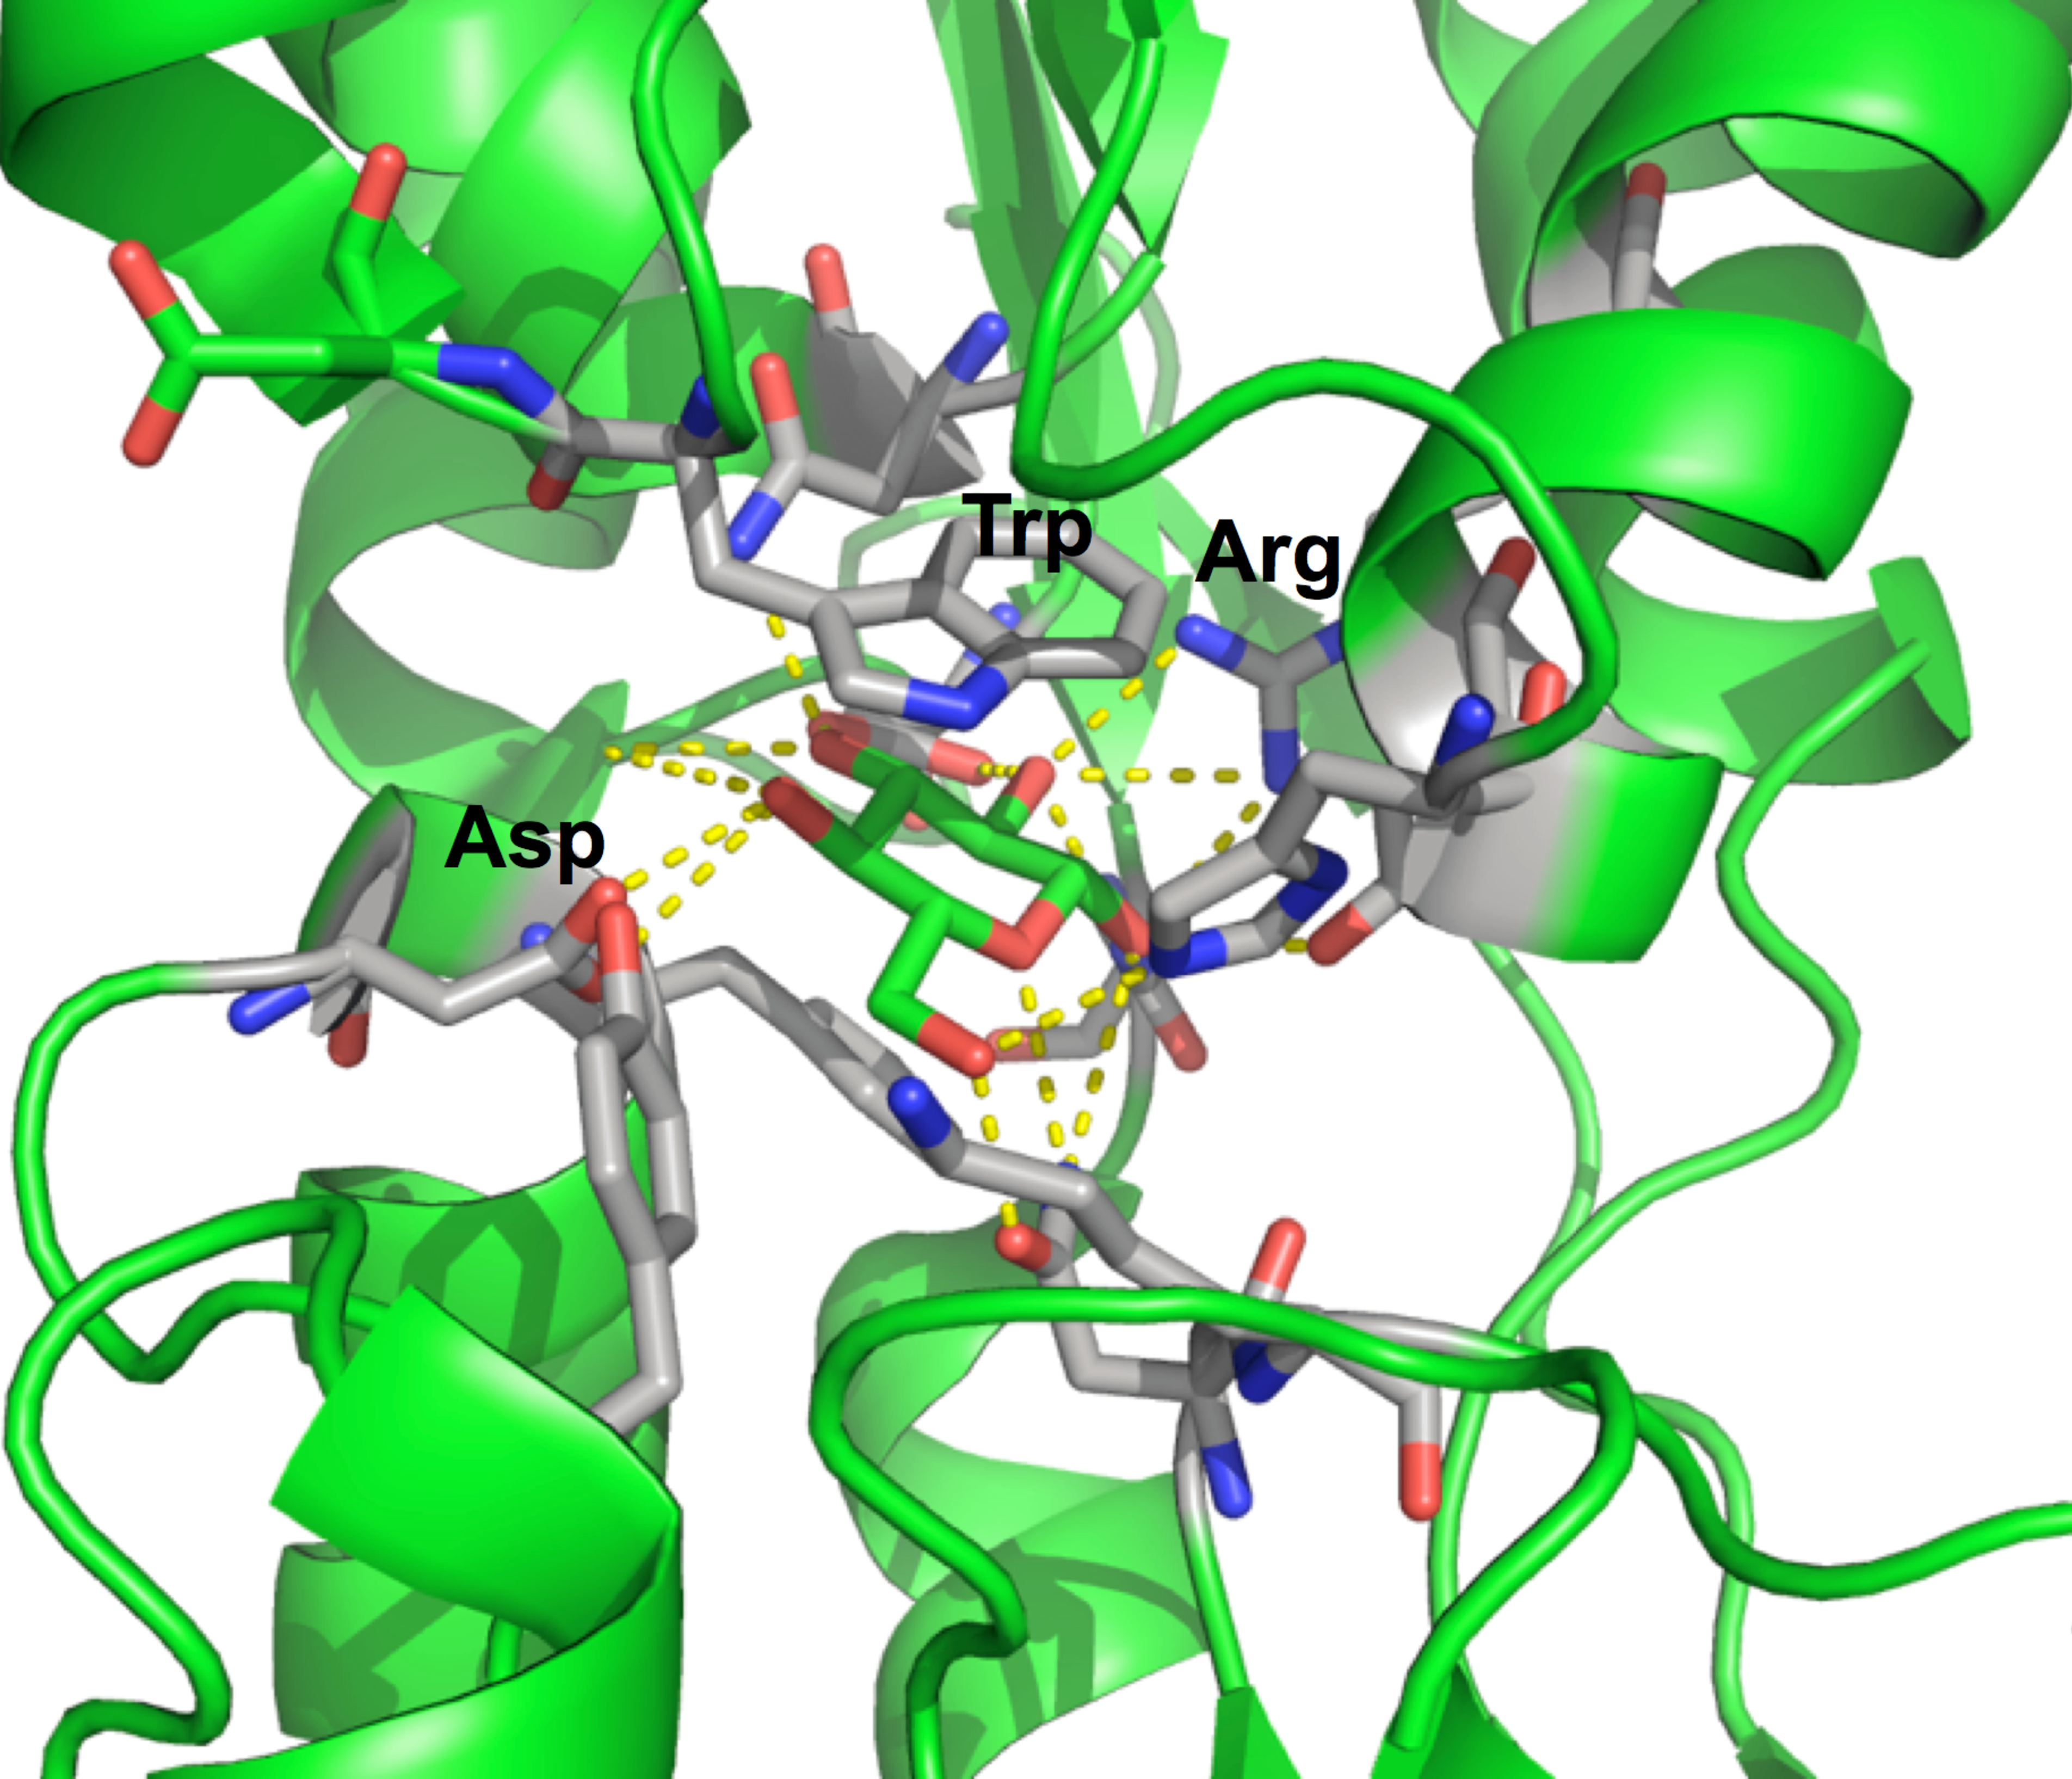
\includegraphics[width=6in]{figures/introduction/sugar_protein_binding.pdf}
 \caption[An example of sugar-lectin binding]{The structure depicts glucose bound to a galactose chemoreceptor protein (Ref: Vyas, N. et al, 1991; Rendered from PDB ID: 2GP).}
 \label{fig:sugar_protein}
\end{figure}

\section{Protein-carbohydrate interactions}
% - Write this section without the cosmic connection
\textbf{Find out what they function as} Carbohydrates are an important component of living cells: they function as a source of energy, building blocks and as recognition elements. Proteins capable of binding carbohydrates are responsible for a variety of functions such cell signalling,REF  antigen-binding, REF and cell-cell adhesion.REF Because of their involvement in many fundamental cellular processes, much research have been devoted to understanding the molecular basis of protein-carbohydrate interactions. 

Carbohydrates are a class of molecules ... that can form polymers via ... A sugar molecule may have different stereoisomers. For example, the sugars X and Y are isomers. Proteins, depending on their function, may have as substrates monosaccharides or polymers of these monosaccharides (oligosaccharides). The structures of a variety of sugar-binding proteins have been solved by X-ray crystallography in the past 20 years. In particular, lectins are a class of proteins that are known to bind monosaccharides.\cite{Rini:1995p2497} An example of a bound glucose in the active site of its protein receptor is depicted in Figure~\ref{fig:sugar_protein}.  The topic of carbohydrate-protein interactions is very complex and is a large field of study in itself.  Here, our discussion will be limited to the binding modes common to many sugar-protein binding interactions for monosaccharides. Detailed reviews of structures of different carbohydrate-binding proteins, and binding of very complex oligosaccharides are out of the scope this thesis and may be found elsewhere. REF

\subsection{Sugar binding sites}
% Summary of the Characterization of the binding pockets
\textbf{How are the sugar sites different from the normal binding sites? I think this should be briefly discussed.}
There are two general types of binding sites: a deep binding site with high binding affinity, or a shallow groove with low binding affinities. The most frequently occurring residues in these sites are aromatic (Trp, Tyr and Phe) and charged residues (Glu and Asp). REF

\begin{figure}
 \centering
 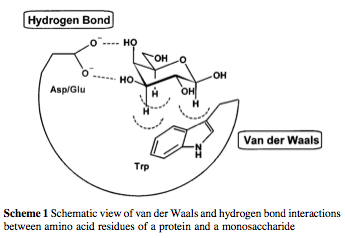
\includegraphics[width=4in]{figures/introduction/sugar_protein_schematic.png}
 \caption[A schematic of monosaccharide-protein binding mode]{A schematic of monosaccharide binding to a binding pocket on a sugar-binding protein}
 \label{fig:sugar_protein_schematic}
\end{figure}

\subsection{Binding modes}
Atomic features of protein-carbohydrate interactions generally possess hydrogen bonding and aromatic stacking interactions.\cite{Vyas:1991p6498} Because sugars have numerous hydroxyl groups (-OH), hydrogen bonds are ubiquitous in sugar-protein interactions. The hydroxyl groups can interact with both polar and charge groups of amino acids including the peptidic backbone.  A monosaccharide is often found to form planar bidentate hydrogen bonds with the carboxylate groups of aspartic and glutamic acids (Figure~\ref{fig:sugar_protein_schematic}).  Moreover, carbohydrate binding is stereochemistry-dependent: the arrangement of the hydroxyl groups around the sugar ring often influences its binding specificity. \textbf{For example} REF
 
Another characteristic carbohydrate binding mode is the nonpolar stacking interactions between hydrophobic faces of the sugar ring and aromatic residues.  The exposed hydrophobic face of certain monosaccharide unit may stack with the planar side chains of aromatic residues (Figure~\ref{fig:sugar_protein_schematic}).  This stacking interaction is thought to be due to the entropically favorable packing of the hydrophobic faces of sugar with aromatic rings, and the enthalpically favorable CH-pi interactions. REF % Other Examples of sugar protein binding. L-arabinose. % look this up

 \subsection{Multivalency in binding}
% Multivalency of sugar binding
% Binding modes of oligosaccharride and monosaccharrides differ.  Mention that oligosaccharride binding is less well-known -- is it?  Found some references for this.
Despite having a low \KD\ (in the millimolar range), carbohydrate-binding proteins have high specificities for their sugar substrates. Although binding specificity is in part influenced by stereochemistry of the sugar, carbohydrate substrates are often capable of forming multivalent interactions, which allows them to achieve their binding specificity.   Talk about multivalency here.  Multiple weak interactions to form one strong interaction.
\textbf{Give a few examples of this ... Antigen binding}

% Molecular simulations of carbohydrates and protein-carbohydrate interactions: motivation, issues and prospects\cite{Fadda:2010p5889} -- this should be moved to the methods or not even mentioned.

% This paper has a pretty good summary of the drug discovery process in the context of CNS. It also has summaries of the experimental techniques used to measure binding affinity\cite{Hubbard:2011fs}

% \subsection{Role of chirality in drug binding}
% Stereoisomerism is important to the activity of molecules. It modulates binding to proteins.
% Two types of stereochemistry
% Constitutional isomers - differs in bonding sequences and connectivity
% Stereoisomers - differs in orientation of their atoms in space, but no connectivity differences.
% Definition of chirality [Add schematic] ... etc
% Molecules with chirality have a non-superimposable mirror image, called an enantiomer.
% A carbon molecule with four different groups has chirality.

% From Lemkul, 2012 review of computer simulations of amyloid simulations
% "From a review of the current literature, it is clear that, despite significant progress, a
% comprehensive study of Aβ-small molecule interactions is lacking. Traditional MD simulations
% must include trajectories of sufficient length that are evaluated for convergence, and multiple
% simulations are strongly recommended for statistical reliability. These criteria have not been met
% in some of the studies reviewed here and represent areas of improvement for all investigators to
% consider. Future investigations on this topic should carefully make use of the features of
% docking, traditional MD, and enhanced sampling techniques like metadynamics, DMD, and
% REMD. Such a combined approach, employing a diverse set of Aβ structures as targets for
% docking and MD analysis, will likely shed light on interactions that can be exploited for the
% development of effective anti-aggregation compounds."

\section{Structure-based rational drug design}
% The purpose of this paragraph is to connect the pharmacological stuff above? So what? what is next? How do we make new drugs or develop better drugs? 
% In order to find new drugs it is imperative to understand the mechanism of action of compounds at the molecular level. 
Structure-based rational drug design is a method that have yielded success in the discovery of lead compounds (Figure~\ref{fig:rational_drug_design}). In this drug discovery paradigm, a target is first identified, with its role in a relevant disease pathway characterized. Then, the molecular structure of the target protein is determined using techniques such as NMR or X-ray crystallography.  By having the molecular structure of target proteins, putative enzymatic active sites or binding sites may be identified.  If the structure of the target is determined in its bound state, protein-ligand interactions can be characterized at the molecular-level. At this stage of the pipeline, high-throughput screening using a chemical compound library can be performed to find lead compounds (e.g. inhibitors) with high binding affinities (low $K_d$) to the binding site. In vitro experiments may be conducted to assess the structure-activity relationship of these compounds.  The information obtained from these experiments can either feedback into the design cycle to find better inhibitors, or be used to guide in vivo experiments.

\begin{figure}
	\centering
	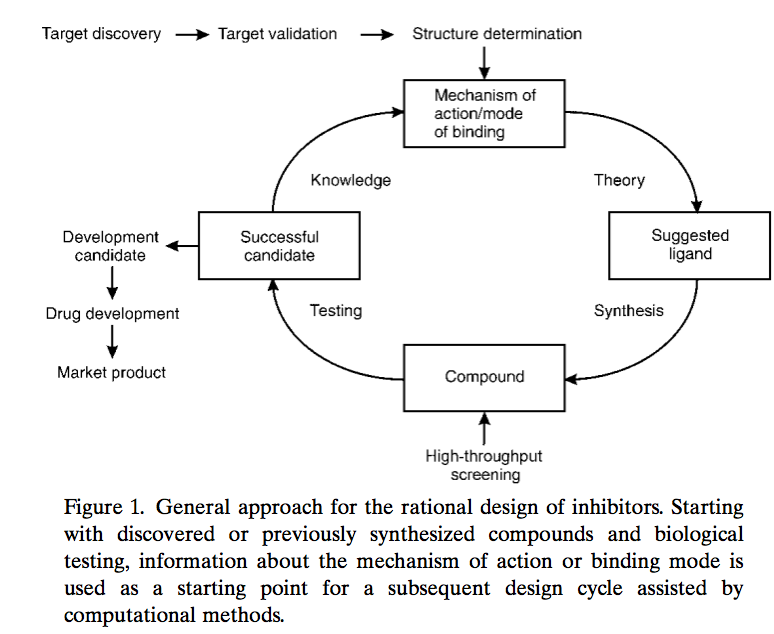
\includegraphics[width=6in]{figures/introduction/drug_discovery_flowchart.png}
	\caption[Schematic diagram of rational drug design]{Schematic diagram of rational drug design. Adapted from\cite{Gohlke:2002in}}
	\label{fig:rational_drug_design}
\end{figure}

\section{Role of computer simulations}
% (Why computational?) Can help us get protein dynamics is important for understanding protein function. We want to understand protein function because we want to be able to design drugs to cure diseases.
% A important application of MD simulation in biochemistry is the predicting of protein-ligand binding free energies.
% In this process, binding free energy of the ligand to its target is 
% \textbf{Computational methods is useful to ...}  One application of MD simulations is in rational drug design. 

In recent years structure-based computer modeling of protein-ligand interactions have become a core component of the modern drug discovery process. For example, computer simulations may be used to predict protein-ligand binding free energies,  a quantity often used to evaluate how well a ligand binds in a high-throughput screening.   Computational docking, where the energetics of binding is typically estimated without accounting for either ligand or protein flexibility may be used to obtain a crude estimate of the binding affinity.  Although docking is fast, its inaccuracy often leads to many false positives. 

Current state-of-the-art computational binding studies use molecular dynamics simulations, which is a much more accurate, but computationally expensive method to predict binding free energies.  With increasingly faster and cheaper computer hardware, molecular dynamics simulations are beginning to play a key role in the rational drug design process. In MD simulations, the protein and its putative ligand is allowed to relax and freely move about in the system, allowing a realistic estimate of the binding free energy to be made. \textbf{MD simulations are .... describe what MD is then go on to say what one can get from it} Simulation trajectories of protein-ligand binding can be used to quantitatively assess whether a chemical change to a compound will produce a more potent drug candidate (e.g.  residues may be ``mutated'' in silico). 

% However, in the case of understanding a specific binding reaction often needed when developing an enzyme inhibitor, the ability to observe the relevant binding events is a low probability event on the timescale achievable by simulations. Therefore, a few enhanced techniques have been developed to accelerate this process.  They are briefly introduced below.

% MD simulations can also be used to rapidly prototype experimental ideas -- for example, one can perform computational alchemy, that is, ``mutate'' residues to test various hypotheses. 

\section{Understanding the molecular mechanism of action of small-molecule aggregation inhibitors}

% How is small molecule binding different from the classical ligand-enzyme binding paradigm? Why is finding small-molecule inhibitors for amyloid is different from finding enzymatic inhibitors. 
Although structure-based rational drug discovery paradigm are well-suited to finding inhibitors of globular proteins such as enzymes, finding small-molecules which may inhibit amyloid formation present many additional challenges. \textbf{The point that I want to make: understanding the molecular mechanism is different because you can't just take an amyloid inhibitor crystallize it with its target and infer how that ligand binds}
\textbf{Need connection}
% These \smi\ often act on species without a well-defined morphology such as those of globular proteins. 
 A high concentration is often required to observe activity (micromolar to millimolar), which suggests that they may be non-specific, and have much weaker binding affinities compared to classical inhibitors of enzymes, which typically have nanomolar \KD's.  Although the concentration of their activity is high compared with classical inhibitors, they are still below co-solvent and osmolarity levels, which suggests these \smi\ may affect aggregation by directly binding to amyloidogenic peptides and / or aggregates.
Hence, their binding equilibria is not described completely by the classical enzyme inhibition models.

Small molecules may inhibit fibril formation, whereas some may prevent only oligomerization, but not fibrillation.   Furthermore, a single small molecule may have activity with different amyloidogenic peptides, suggesting that there are generic mechanisms at play. \textbf{Where is this going?}

% They are able to be active at much lower affinities. Their binding site on amyloids are often not know. Amyloid aggregates present a binding surface, so it is not unexpected that these small molecules do not bind in one specific binding pocket.

\textbf{Why is molecular dynamics particularly useful here? Say at very high level what MD is. Refer to the section for the detailed methods.  Then connect to the review of MD studies of small-molecule amyloid binders/inhibitors below. Splice out some of the stuff on dyes from the earlier sections to move to here?}

% What is the evidence for direct binding? NMR studies indicate direct binding activity for several small molecules.\cite{XXX EGCG paper nature 2007}. EGCG was found to directly bind to alpha-s and Abeta.

\section{Computational studies of amyloid inhibition by small molecules}
% In recent years, molecular dynamics simulations have been intensively used to investigate the molecular basis of the structure and stability of amyloid fibrils. 
% 
% MD simulations of Congo red binding have been done with the protofibril-like crystal structure composed of the segment GNNQQNY.\{Wu, 2007 \#621\}
% 
% A recent simulation study of an N-methylated peptide with A$\beta$16-22 models of amyloid aggregates has provided insight into the possible mechanism of action of peptide inhibitors of amyloid formation.\{Soto, 2007 \#597\} This peptide inhibitor was shown to preferentially bind monomers to form dimers, possibly acting to inhibit fibril formation by sequestering monomers. However, peptide-based inhibitors have poor pharmacological profiles as they are actively broken down by proteases in the stomach and are difficult to transport across the blood-brain barrier. In addition, these peptide inhibitors specifically target A$\beta$ and thus do not have the potential to treat multiple amyloid diseases.

% Simulations thus far which have examined small molecule binding with peptides that are truncated (such as that of A$\beta$(12-28) and A$\beta(16-22)$) forms of the full-length peptides of Abeta (AD) or alpha-synuclein or IAPP. If not the the shorter peptide, studies typically employed forms with structure such as the protofibril of Abeta40 or Abeta42 both of which have SSNMR starting structure coordinates.

Although many \smi\ were found to have activity in affecting amyloid formation, only a limited number of them had their binding mechanism examined by MD simulations. In this section, we review previous studies of MD simulation studies of the binding of small molecule inhibitors of amyloid formation that were published between the years of 2007 to 2013 (the time of writing of this thesis).

% Notes: What exactly should I cover in my reviews?
%Explicit solvent? Is this too much detail?
%Extensive simulations? Simulation times?
%Conventional MD? Special tricks were used?
%Force field?
%Concentration / molar ratio
%statistics?

\subsection{Dye binding}

An early study of an amyloid dye and inhibitor phenol red binding with NFGAIL protofibril.\cite{Wu:2006gx} Phenol red was found to bind non-specifically to the protofibril, that is, it did not adopt consistent binding modes (confusing ... what? find better words). % a dye or a polyphenol?

% Congo Red:
In 2007, Duan et al.\cite{Wu:2007p361} performed short simulations of the protofibrils of GNNQQNY in the presence of two molecules of congo red, where they found that CR adopted two main binding modes: CR was either bound either in the grooves of the fibril, parallel to the long axis of the fibril or in between two peptide strands, perpendicular to the long axis. Based on contact binding analysis, the main driving force for the binding appears to be hydrophobic interactions. Based on their results, they speculated that by binding in the grooves at the surface of the amyloid protofibril, CR may block fibril growth along the $\beta$-sheet stacking direction. Note: This study shows (really? they showed that? how?) that disrupting stacking could lead to disaggregation:  Wu, C.; Lei, H.; Duan, Y. Biophys. J. 2005, 88, 2897-2906. 

In a follow-up study, Shea et. al. REF used a similar protocol of the study reviewed above to study the binding of CR with protofibrils of full-length \abeta40.\textbf{And what was the conclusion?}

% ThT 
Molecular mechanism of ThT binding was probed in recent years by several simulation studies. In a 2011 study by Wu et al.,\cite{Wu:2011fd} a comparative study of the binding of PIB and ThT was examined with protofibrillar models of \abeta40\ and \abeta42\ derived from SSNMR studies. Both dyes were observed to bind at the tunnel of the fibril (\textbf{what is this tunnel?}). Charge-charge interactions between ThT and protofibrils did not appear to play an important role in binding. This was found to be the key reason explaining why the removal of charges from ThT made PIB binding more favorable than ThT binding. For \abeta40, in agreement with experimental observations of multiple binding sites and binding affinities, ThT and PIB bound to multiple aromatic or hydrophobic grooves, loops, and edges with different binding ratios and affinities.   Energetic analysis show that stabilizing forces are the van der Waals term and surface hydrophobic interaction term, whereas electrostatic interaction terms were unfavorable. Binding modes to \abeta42\ were found to be similar to \abeta40, except dye molecules were able to enter the channel located at the loop of A$\beta$(17-42) cross-beta-subunit, but not the channel on \abeta40.

% [Sketchy study] Another early study of 9,10-Anthraquinone suggests that intercalation and interactions between the backbone of peptides destabilize oligomer formation.\cite{Convertino:2009ce}

\subsection{Polyphenols}

Several MD simulation studies have studied the binding of EGCG with monomers and fibrillar forms of A$\beta$. 

A combined MD and NMR study by Wang et al in 2010\cite{Wang:2010p5887} suggested that binding modes of EGCG with monomers (XXX) of \abeta42\ is modulated by ligand stoichiometry. The study concluded that both hydrogen bonding and hydrophobic (aromatic) interactions are important for binding of EGCG.\textbf{Expand on this - what exactly was the point of this study?}

A study by Sun et al in 2011,\cite{Liu:2011ka} (\textbf{did this study build on top of the other one?}) later suggested that EGCG binds a monomer of Abeta42 XXX (this is repetitive ... how did this study differ from the Wang study?).  MM-PBSA analysis suggested that nonpolar interactions contributed more than polar interactions to its binding modes. Hydrogen bonds were formed with the main chain (so?)  The transition from the initially helical conformation to $\beta$ was prevented by increasing the ligand:peptide molar ratio of ECGC from XXX to 10:1. [I find this study sketchy. Note that this group also performed the sketchy trehalose study.]

% Binding of EGCG with monomers of Abeta42 were conducted at different concentration of EGCG molecules by Liu et. al.\cite{Liu,2011} 
% Forcefield was GROMOS. They ran 3 repeats per system, each system were ran for 300 ns.  
% The results were averaged over the trajectories. 
% No unbinding / binding statistics were observed over the course of the simulation (why not? Perhaps EGCG has a much higher binding affinity than inositol) -- see figure where the number of monomer - EGCG contacts were increasing over time.  Claims that binding prevented the monomer from transitioning from alpha to beta, but if you look at the numbers in the table, the only significant difference is the number of residues in beta. And even then, its not that different between no EGCG and 0.04 mol/L system.  I guess if the molecules has a much higher binding affinity, one would need to simulate for much longer to get binding statistics.   Because there were no unbinding events, this was a nonequilibrium simulation.  Of course if one set had molecules bound all the time that it is likely the conformational equilibrium of the monomer is different from that of the set without anything bound.

Binding of morin molecules with the protofibril form of \abeta42\ was examined by Lemkul et. al. They observed that morin hydrogen bonds with ... based on one or two snapshots of binding. In a follow-up study, Lemkul et. al. performed simulations of dimers of \abeta42\ peptides. Morin was not observed to bind directly to the CHC sequence, but rather to residues flanking it, suggesting that Abeta aggregation inhibitors may act at indirect or allosteric sites to influence peptide structure. Their overall conclusion of morin's mechanism of action is that it binds abeta42 to alter its tertiary interactions as it aggregates, and thereby preventing \abeta42\ monomers from forming stable hydrophobic nuclei (I think these conclusions are far-fetched). \textbf{Politely make the following point - No statistics. No binding modes other than the anecdotal evidence of what it was bound.}

\subsection{Nonsteroidal anti-inflammatory drugs (NSAIDs)}
Ibuprofen and Naproxen are NSAIDs, typically used for pain relief, have also showed in vitro activity as an amyloid inhibitor. In a series of MD simulation studies, Klimov et. al. probed the binding mechanism of these compounds with the SSNMR model of the fibrillar aggregate of \abeta40\. REFS Their results suggested that NSAIDs predominantly bind via hydrophobic interactions, at the grooves of the edges of protofibrils.  They suggest that this a possible way by which these molecules may prevent fibril formation.
% replica exchange was used to probe binding of both molecules with the protofibril of Abeta40 (the ssnmr structure).

\subsection{Other small molecules}
Trehalose is a disaccharide that has been shown to affect the aggregation of \abeta40\ in vitro. REF Although it works in vitro, its vivo pathway is not by acting as an amyloid inhibitor. REF Liu et. al in 2009 performed explicit solvent simulation of trehalose molecules with peptides of Abeta(16-22).  The GROMOS forcefield was used for the modelling of the peptides and trehalose molecules.  Trehalose prevented the oligomerization of the peptides in their simulations. Furthermore, the presence of trehalose decreased hydrophobic contacts and interpeptide hydrogen bonding. Based on their results, it was speculated that trehalose may prevent the nucleation and elgonation of Abeta16-22 oligomers via the preferential exclusion effect.   

\textbf{Note to self - could it be because of differences in force field that I am getting such different results from the trehalose study?  Or is it a lack of convergence?  (On their part?) Or both?  Is the OPLS-AA force field much stickier than the gromos force field?  Also GROMOS favors the formation of beta sheets so its possible that, they were able to see beta sheet formation over the course of their simulations?  [Sketchy study]}

Convertino et al. 2009 comparatively examined the effect of AQ and XXX on the aggregation of peptides of Abeta(16-22) using implicit solvation simulations.  AQ form of the ligand was found to disrupt the oligomer the most.  The AQ ligand has both hydrogen bonding groups and aromatic groups caused the most disruption. The authors found that AQ interacalated between peptides by forming hydrogen bonds with the peptides. However, it was not clear whether competition for peptide hydrogen bonding by AQ led to the disaggregation or did the peptides dissociated before the binding occurred. [sketchy study]


% Could lead to a number of defense questions:
% Do you think it could be the preferential exclusion effect for inositol?
% Why do you think different force fields led to such different results?
% Can you speculate how force fields could influence your results?  If you had different force fields ... what would you expect to get the same results / conclusions again?

% REF: Liu, F.-F., Ji, L., Dong, X.-Y., and Sun, Y. (2009) Molecular insight into the inhibition effect of trehalose on the nucleation and elongation of amyloid �-peptide oligomers. J. Phys. Chem. B 113, 11320!11329

% Garcia et al. studied
% At the time of writing, recent studies of anti-amyloid agents in literature includes galantamine
% Some docking studies were also done. For more detail on this, see the recent review by Lemkul et al. http://www.ncbi.nlm.nih.gov/pubmed/23200245

% \subsection{Comparisons of literature studies}
% In summary, simulation studies suggest that both hydrophobic interactions (involving aromatics) and hydrogen bonding interactions appear to be involved in the binding mechanism of known in vitro small molecule inhibitors.  Several studies (which one) observed that peptide - peptide intercalation by the small molecule ocurred via hydrogen bonding interactions.

% Gaps ... However, there are a number of issues with the current studies. Studies are not comparative. Some studies use implicit solvent only.  Each of the studies reviewed above use a different force field. Concentration dependence rarely looked at. High concentrations were used for both peptides and ligands. All studies seem to �confirm� the in vitro studies for the ligand of interest.
% No systematic comparisons of monomers, disordered oligomers and beta oligomers. So if a study is studying binding to beta oligomers, then it concludes that the ligand of interest binds at surfaces, and therefore works by preventing protofibril stacking. If binding to monomers, slight differences in conformational ensembles in monomers with and without ligands results in the study concluding that it affects monomers.

% And then say bam our study is complete �  we need to be as complete as possible for our study. 
% Thus far no enhanced sampling methods used with explicit solvent. Studies do not attempt to converge the monomeric peptide ensemble.

\section{Thesis objectives}

% How to tie this figure into this section?
\begin{figure}
\centering
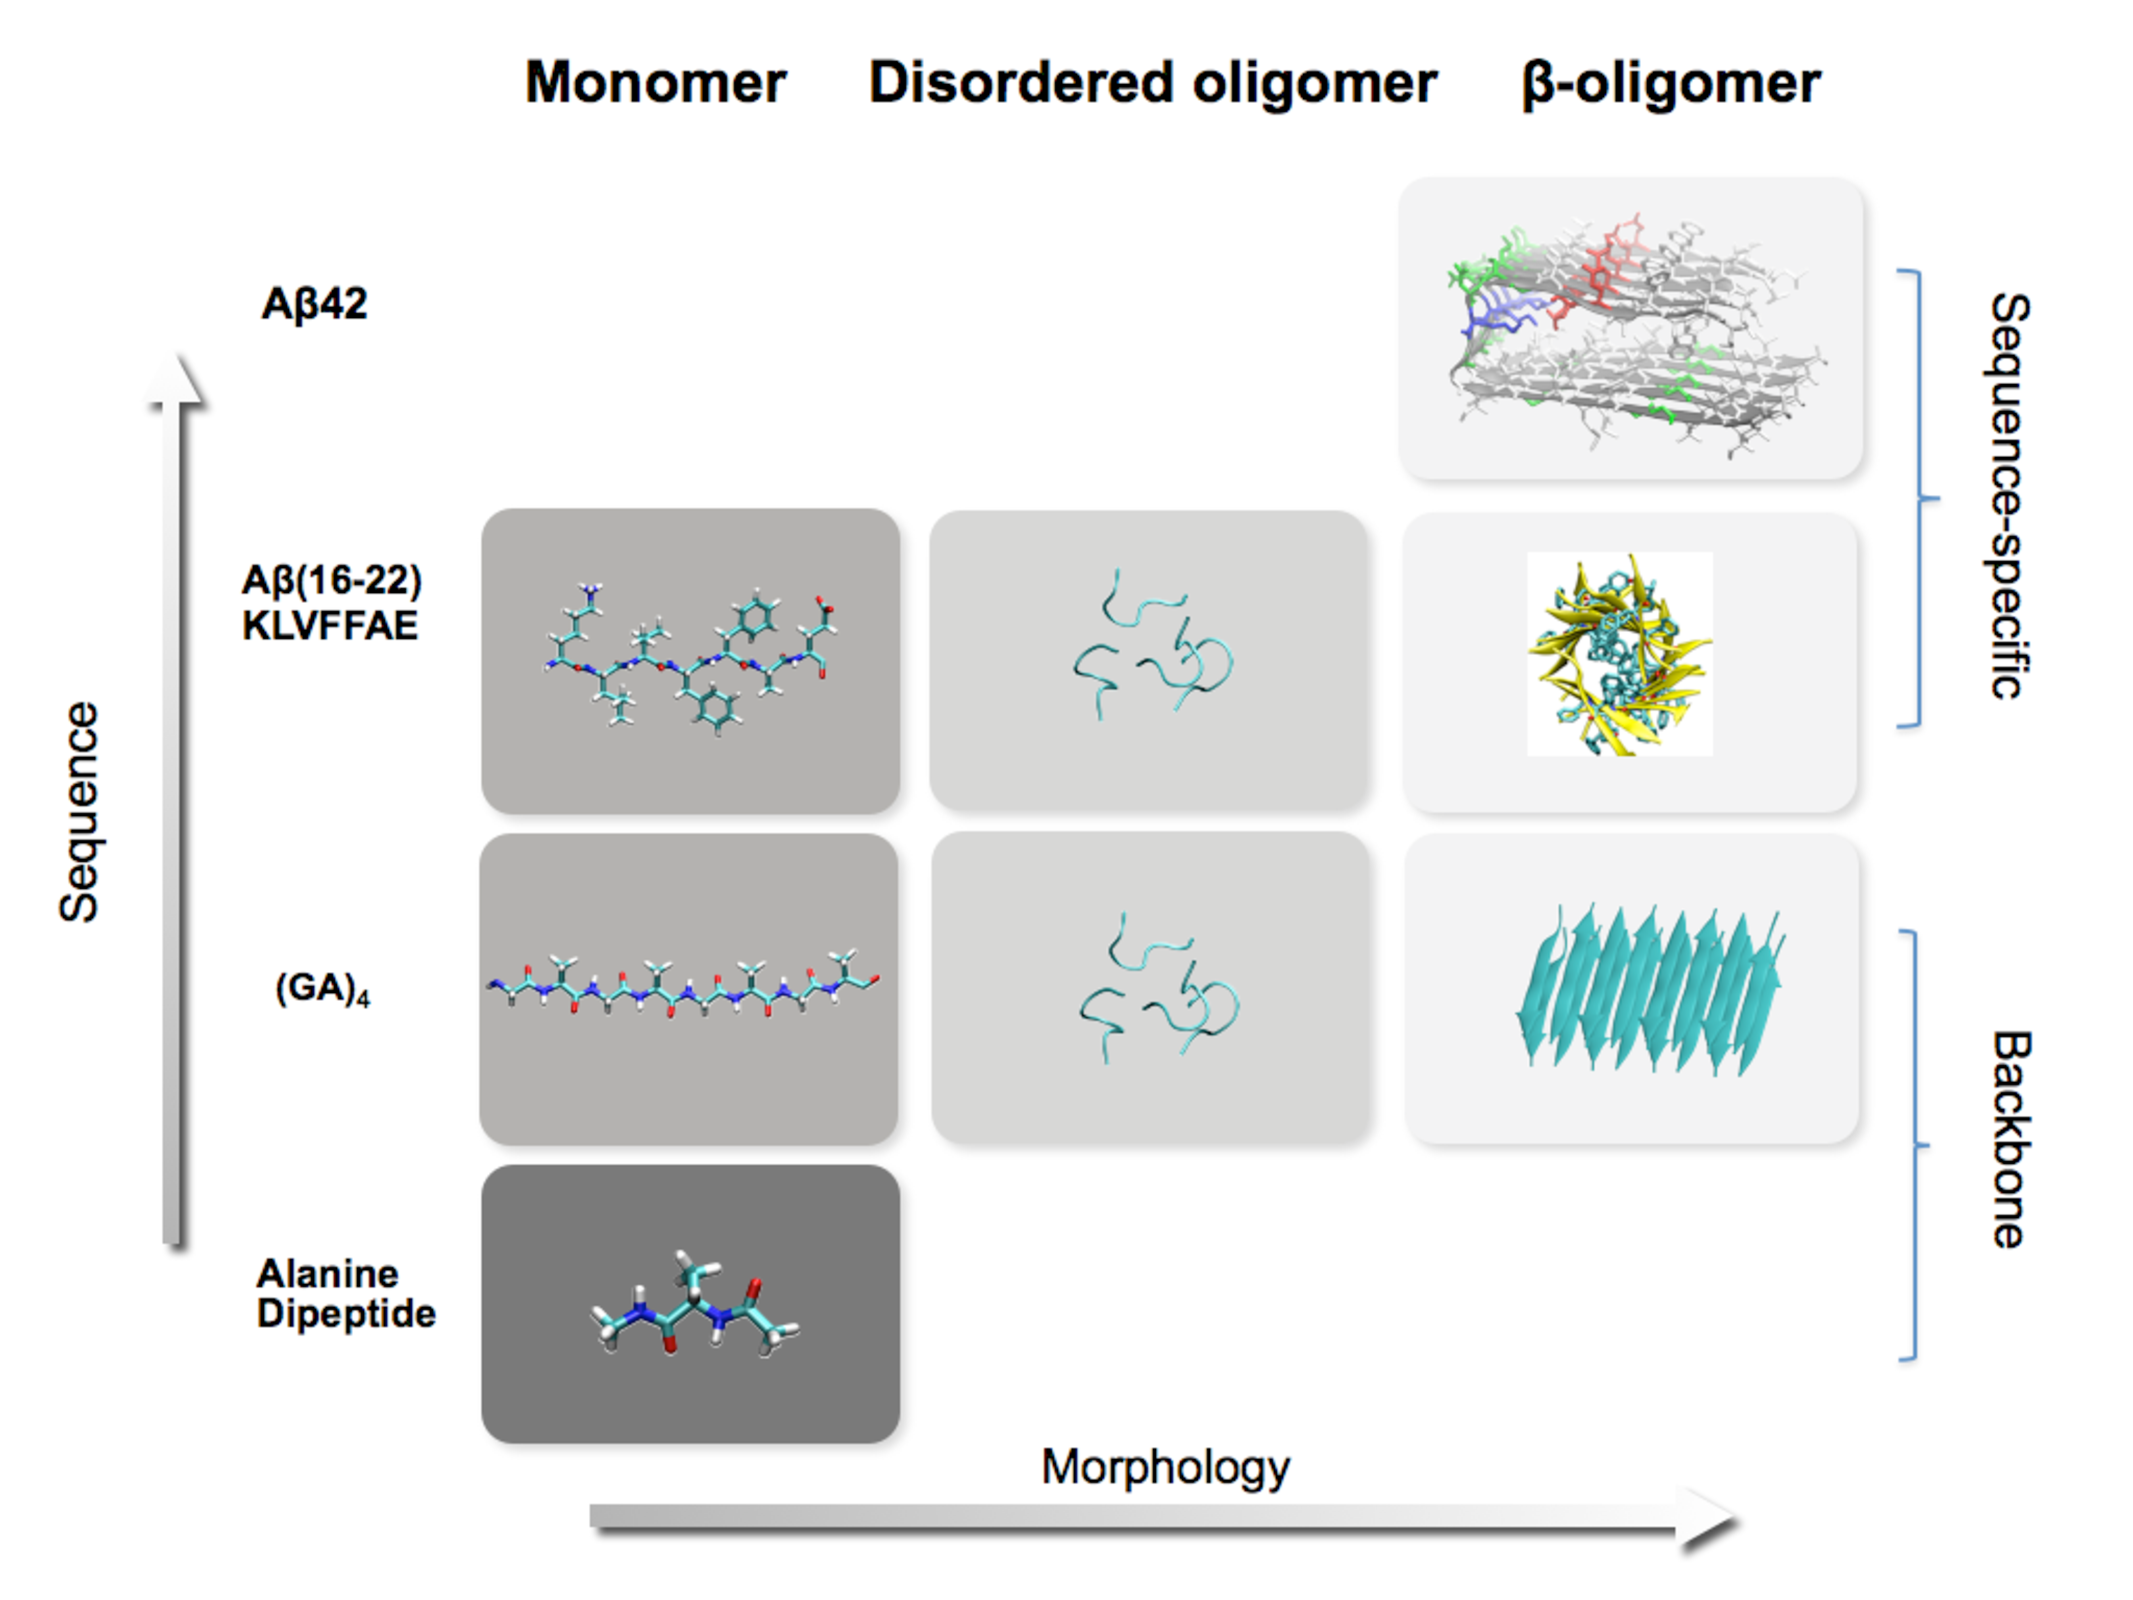
\includegraphics[width=6in]{figures/introduction/matrix.pdf}
\caption[Thesis Rationale]{Using a reductionist approach, we progress from examining model amyloidogenic peptides and aggregates to more complex systems involving the full-length A$\beta$42 peptide.}
\label{fig:rationale}
\end{figure}

The central hypothesis of this research is that inositol exerts its effects through direct binding to one or more of the monomeric, aggregated, or fibrillar forms of amyloidogenic peptides and proteins.   

Multiple sources of experimental evidence have demonstrated the existence of species that are morphologically distinct from fibrils in the amyloid aggregation pathway.6, 13, 29 At least two intermediates on pathway to fibril formation have been observed: oligomers and protofibrils. These species together with the monomer and fibrils, constitute a possible pathway by which A$\beta$ aggregates to form fibrils. 

In order to characterize the molecular mechanism of action of inositol, it is imperative that the interaction of inositol with various aggregate species be examined. To this end, I will carry out systematic comparative studies of amyloidogenic peptides and their aggregates of increasing sequence and composition complexity and characterize the respective role of specific interactions of inositol with the backbone and sidechains. Inositols have been shown to have stereochemistry-dependent activity in vitro and in vivo.18, 20 Chiro-inositol is a stereoisomer that was shown to be inactive in inhibiting amyloid formation. Thus, I will comparatively study chiro- and scyllo-inositol with each of the aggregates in the pathway to determine the stereochemical basis of the activity of inositol.

\section{Thesis Organization}
Chapter 1 introduces the work presented in this thesis in the context of the field. Chapter 2 introduces the main methods used in the work in the thesis.   In chapter 3, we systematically examined the binding modes of inositol with simple models of amyloidogenic peptides. Next, we examined binding with KLVFFAE, .... Chapter 5 details studies with the protofibrils of the full-length A$\beta$42. In Chapter 6 we demonstrate the general applicability of our methodology developed in this thesis by applying similar MD simulation approaches to examine protein - carbohydrate binding. Chapter 7 provides discussion, suggestions for future work, and perspectives.

\addcontentsline{toc}{section}{Bibliography}
\bibliographystyle{plain}
\bibliography{introduction}

% To determine the effect of inositol on the structure and thermodynamics of the self-aggregation of different amyloidogenic peptides.

%\subsection{Study Design}
%
%Simulation challenge - The structural disorder of the peptides involved poses a challenge for obtaining converged properties from MD simulations. To date, few studies have attempted to provide statistically meaningful results pertaining to general mechanisms of protein self-aggregation and amyloid formation. Furthermore, despite the abundance of MD studies of A$\beta$, few studies have systematically examined the mechanism of action of small molecule inhibitors of amyloids
%
%% If you mention brute force ... most scientist in the audience won't understand
%For sampling, we exploit conventional MD simulation techniques because simulation approaches used for understanding enzyme-ligand binding is not applicable. Conventional MD simulations were combined with many repeated independent replicas to obtain statistics on the binding equilibria. We use many repeat simulations - why ? We can observe binding and unbinding events within several nanoseconds. This is an approach that is typically used to trivially parallelizing simulations to speed up sampling. Because inositol acts at higher than normal (what do you mean by this) concentrations (in vitro), we were able to approach this problem using a ``bulk" approach, by examining binding between multiple molecules of inositol with different amyloid aggregates. Inositol's interactions are weak (but I shouldn't be stating this as an assumption.. because 90\% of inositol's interactions may be weak, but the 10\% which are not may be the ones that induce its activity).

% Instead, we use conventional MD simulations and repeats of independent simulations to determine the binding modes, and binding equilibria of inositol with amyloidogenic peptides and aggregates of A$\beta$.
%of both increasing sequence and structural complexity.

% Two important lines of evidence support the above hypotheses. First, preliminary experimental data from the McLaurin lab are showing that in addition to \abeta42, inositol can also inhibit superoxide dismutase (an amyloidogenic protein involved in amyotrophic lateral sclerosis), $\alpha$�-synuclein (Parkinson's disease), and poly-Q (Huntington's disease) amyloid assemblies in a similar manner to \abeta42\ (J. McLaurin unpublished data). Since all amyloid structures have the cross $\beta$-sheet structure in common, their findings suggest that inositol is capable of binding the polypeptide backbone. Secondly, our own systematic MD study of inositol with alanine dipeptide, a model of the peptidic backbone, has demonstrated that inositol binds to the peptidic backbone through hydrogen bonding interactions (See Section 5.1 below). 


% AD
% Treatment - harder to treat - lack of biochemical understanding of what causes disease, which makes it difficult to develop drugs for; lack of good diagnostic methods because treatment may not be effective at end stages of the disease where brain function won't e able to be rescued.
% Diagnosis - hard to diagnose
% AD is difficult to diagnose. It is often not apparent that someone has AD until they exhibit symptoms severe enough to interfere with daily life or occupation. 

% Amyloid hypothesis - our best guess at what causes AD and provides the best guess at what we should be targeting. 
% Abeta Amyloid thus far provides the best clue to the molecular basis of AD, and thus a promising pathway to a cure for AD.

% In some individuals without dementia symptoms may have as much plaque as another with severe AD. Synaptic loss can be used as a measure of disease progression. 

% Perhaps use this as a transition into the general discussion of amyloid formation and structure -- not only specific to Abeta.
% Furthermore, amyloid have also been known to play beneficial roles in certain living systems. REF
% Increasing awareness of the amyloid state of proteins, and interest grew in amyloids because of their role in a variety of devastating human diseases.

% Fibrils

% In this section I will talk about how amyloid aggregation is thought to work. Introduce the thermodynamic model for understanding fibril formation.

% Understanding amyloid inhibition in the context of the framework of traditional enzyme inhibition mechanism
%[Challenges of developing small molecule for amyloid inhibition] Structure-based drug discovery approach developed to target folded proteins such as enzymes cannot be directly applied to discovery of small molecules which targets amyloid formation.  A$\beta$ peptides are completely disordered. Because the A$\beta$ amyloid aggregate pathway encompasses a variety of species, some of which are disordered, a single conformation cannot be assumed for binding. Furthermore, structural information of amyloidogenic species lags behind those of enzymes, which tends to be globular proteins amenable for X-ray crystallography. This means that the putative binding sites are not known. 

% We don't know if a small-molecule like inositol acts by binding. Do the ligands bind? If they bind, we do not know where they bind. It is experimentally challenging to identify the binding sites using available techniques such as SSNMR, NMR, and X-ray. 
% Although there are some data other there with experimental data, we cannot yet obtain fully atomistic detail on the interactions between the ligands and proteins.

% Because amyloid is a group of different species, where the structures of which are largely unknown, we don't know (and we cannot assume) which aggregate species along the amyloid aggregation pathway that inositol may interact with. We want to examine representative species within the aggregation pathway, that is, monomers, disordered oligomers, and fibril like aggregates. Furthermore, we cannot assume putative binding sites - that is these binding sites are not known a priori. Unlike the case with enzymatic inhibition, a single bound molecule is unlikely to inhibit fibrillation. Instead, amyloid aggregates such as fibrils present surfaces for binding.

% Furthermore, amyloid inhibitors are found to be very weak binders.  A key question is how do non-specific inhibitors act as a drug? 

% How do we approach this with MD simulations?
% In AD, there is the added challenge of the drug being able to cross the brain barrier, while remaining non-neurotoxic. What kind of drugs cross the BBB? Typically hydrophobic drugs.

% We also do not know what the binding site looks like, where it is located on these structures.

%% However, most of these studies were focused on A$\beta$ and large A$\beta$ aggregates,\{Fawzi, 2008 \#553;Esposito, 2008 \#567;Sgourakis, 2007 \#609;Wei, 2006 \#656;Tarus, 2006 \#628 Karsai, 2006 \#658\} and thus, were computationally limited by the complexity of the molecular systems.
%
%% Here describe in detail how I designed my study to circumvent the challenges presented by the amyloid inhibition problem, and the limitations of MD simulations. At this point, clearly explain and discuss my study design and rationale. 
%% (Don't know binding? binding site? which structure does it binding? how does it binding? "binding mechanism")
%
%
%Although amyloid fibrils of different peptide sequences share the overall cross-beta, there are specific differences in their surface properties due to their amino acid composition. Hence, we look at different species of different peptides.
%
%We took a reductionist approach to solve this problem. Beginning with the simplest model of an amyloidogenic peptide, we systematically examine binding of inositol with systems of both increasing sequence and structural complexity.
%
%% First started with the simplest peptide of relevance, the alanine dipeptide. We started with the alanine dipeptide to look at backbone interactions. 
%We wanted to isolate the problem to something simple to examine the backbone binding mechanism of inositol. Because inositol had many hydrogen bonding groups, and it is shaped like it is geometrically suited to bind the peptidic backbone. Why did we first choose to look at the backbone? Because it is the common element in all polypeptides, and the common cross-beta where the backbone of polypeptide chains are organized in the same manner in the structure of amyloid fibrils suggests that backbone plays an important role in amyloid formation. We examine aggregates of varying sequence and structural complexity. By examining a simple beta-sheet forming peptide, (GA)4, an amyloid inhibitor may bind to a simple amyloidogenic peptide. An illustration of this approach is shown in Figure~\ref{fig:rationale}.


%\subsection{Choice of Model Systems}
%Following the approach of studying systems of increasing complexity, we have chosen the following peptides and sequences: (1) Alanine Dipeptide; (2) (GA)4; (3) KLVFFAE; (4) SNNFGAIL; (5) Aβ40/42. Amyloid-forming proteins involved in disease, such as Aβ, Tau (Alzheimer's) or hIAPP (diabetes), are often many residues in length and high in sequence complexity, which renders the collection of meaningful statistics from large-scale computer simulations of these protein aggregates difficult. However, many of these longer sequences have been found to have shorter segments that preserve the amyloidogenicity and cytotoxicity of the longer parent protein.30, 31 These shorter peptides not only have been shown to retain the physiochemical properties for studying general mechanisms of amyloid formation experimentally, but also are much simpler systems suitable for detailed computational studies.
%
%4.4	Alanine Dipeptide
%	Alanine dipeptide (N-acetyl-L-alanine-N'-methylamide or AcAlaNHMe) is a minimalist model of the peptidic backbone with its two backbone dihedral angles (φ,ψ) as its significant degrees of freedom. The dominant conformations of its conformational equilibrium span all possible dihedral angles representative of α-helices and β-sheets in (Figure 1A). Due to the simplicity of alanine dipeptide, all relevant local peptidic backbone binding modes of inositol can be explored efficiently computationally.
%
%4.5	GAGAGAGA
%	An octamer with repetitive sequence involving only nonpolar side-chains, (GA)4 is the simplest amyloidogenic peptide32 of relevance to study the interaction of inositol with the peptidic backbone. GA is a commonly occurring sequence motif in the β-sheet forming (crystalline) domains of a variety of spider silks.33 The tetramer GAGA is a part of the B. Mori silk fibroin, which is found to contain β-sheet structure.34 The repetitive nature of (GA)4 and its low sequence complexity allow simulations to be computational tractable and thus, permits timescales needed to determine the effects of inositol on amyloid aggregation in a statistically meaningful way. Finally, the simplicity of (GA)4 allows the detailed examination and dissection of the different possible types of inositol-peptide interactions. 

%4.6	KLVFFAE
%	The peptide KLVFFAE, a segment spanning residues 16 to 22 of Aβ1-40 and Aβ1-42, has been well studied both experimentally and computationally.35-38 KLVFFAE is the central hydrophobic core thought to be important in full-length Aβ assembly and is affected by four AD causing mutations: A31G (Flemish), E22Q (Dutch), E22K (Italian), and E22G (Arctic). This peptide not only contains side chains with more bulk, but also those capable of forming charged and aromatic interactions. The protofibrillar structure has been shown by SSNMR to have anti-parallel β-sheet organization with possible parallel stacking of the β-sheets.36 

% 4.7	SNNFGAIL
%	hIAPP(20–27) (SNNFGAIL) is an octameric segment of the 37-amino acid residue hIAPP polypeptide and is both amyloidogenic and cytotoxic.39 Pancreatic amyloid in humans forms through the aggregation of islet amyloid polypeptide (hIAPP). hIAPP-derived amyloid is found in more than 95% of type II diabetes patients and is believed to be directly involved in the pathogenesis of the disease. The peptide SNNFGAIL is different from KLVFFAE in that it is an amphipathic peptide where SNN is polar and FGAIL is nonpolar.39 Thus, the protofibrillar structure formed will likely have different surface properties despite sharing similar backbone secondary structure.

%4.8	Full length Aβ40 or Aβ42
%	Inositol does not necessarily act on the shorter peptide models and their aggregates. To address this possibility, I will study inositol with the Aβ peptide and aggregates. The monomeric, oligomeric, and fibrillar structures of Aβ40 and Aβ42 have been studied both experimentally and computationally.4, 16, 40-45 Thus, I will utilize the structural data available to construct oligomeric and fibrillar species and comparatively analyze the interaction of chiro- and scyllo-inositol with these species.